\documentclass[12pt]{article}
\usepackage[UTF8]{ctex} % Required for inserting images
\usepackage{longtable}
\usepackage{geometry}
\usepackage{array}
\usepackage{tabularx}
\usepackage{graphicx}
\usepackage{float}
\usepackage{listings}
\usepackage{xcolor}
\usepackage{amsmath}
\usepackage[hidelinks]{hyperref}
\usepackage{titlesec}
\usepackage{tocloft}

\geometry{left=1.5cm,right=1.5cm,top=1.5cm,bottom=1.5cm}

% 定义新的section级别
\setcounter{secnumdepth}{4}
\setcounter{tocdepth}{4}

\titleformat{\paragraph}
{\normalfont\normalsize\bfseries}{\theparagraph}{1em}{}
\titlespacing*{\paragraph}
{0pt}{3.25ex plus 1ex minus .2ex}{1.5ex plus .2ex}

\newcommand{\subsubsubsection}[1]{\paragraph{#1}\mbox{}}

\begin{document}

\begin{titlepage}
    \centering
    \vspace*{\fill}
    \bfseries\Huge
    Matlab图像处理大作业\\[1cm]
    \Large
    无23尤忆晨\\[0.5cm]
    2022010576\\[0.5cm]
    2024/8/28
    \vspace*{\fill}
\end{titlepage}

\tableofcontents
\newpage

\section{基础知识练习题}

\subsection{MATLAB工具箱}
输入help images得到:
\begin{figure}[H]
    \centering
    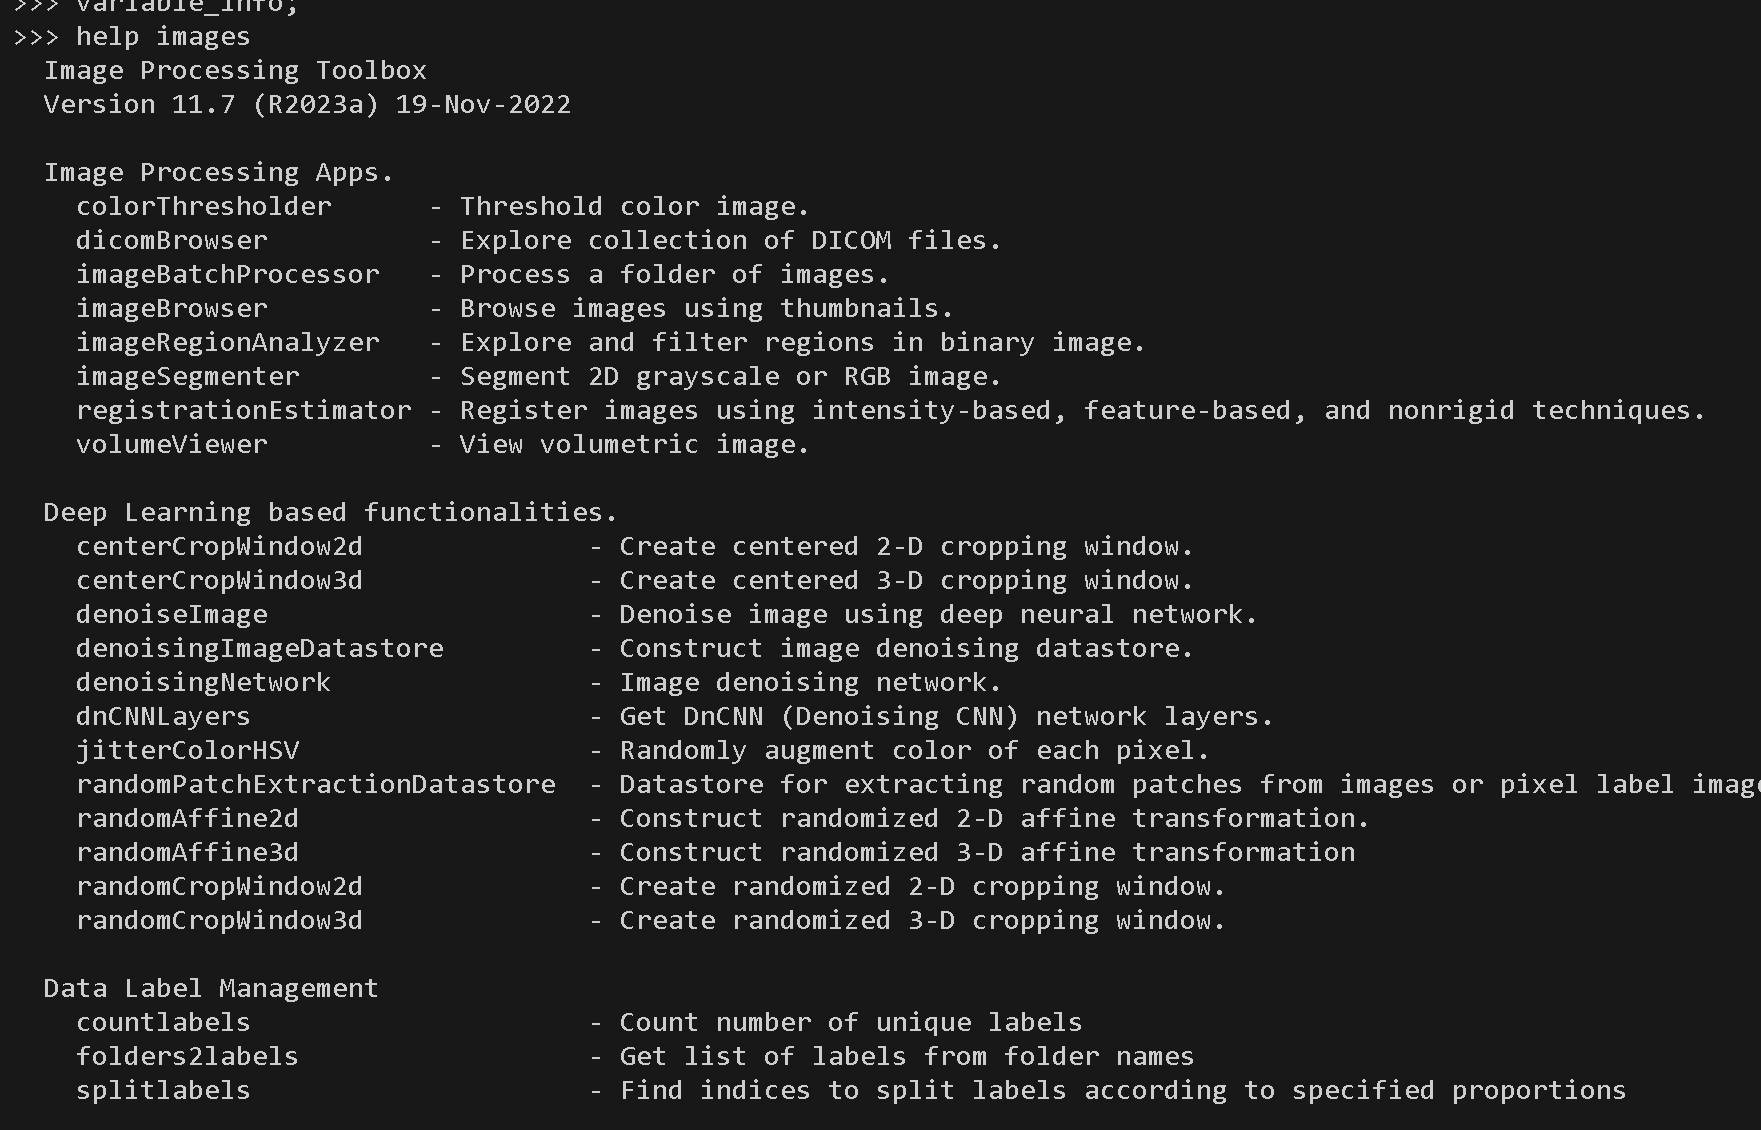
\includegraphics[width=0.6\linewidth]{help.png}
    \caption{所有函数}
\end{figure}

\subsection{完成以下处理}

\subsubsection{绘制红色圆}

\begin{figure}[H]
    \centering
    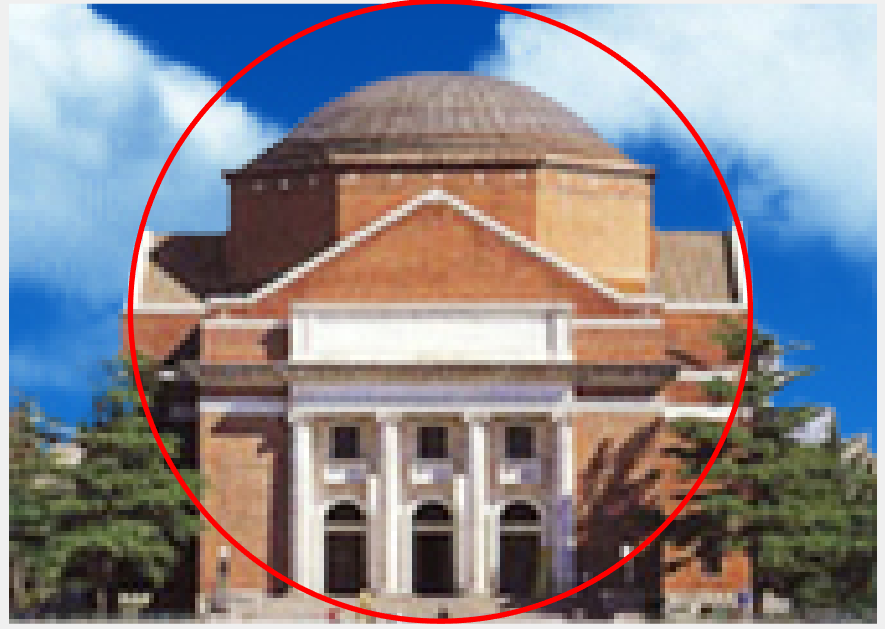
\includegraphics[width=0.6\linewidth]{1_a.png}
    \caption{绘制红色圆}
\end{figure}

\subsubsection{绘制棋状黑白格}

核心代码:
\begin{lstlisting}[language=matlab]
    % 计算每个棋盘格的大小
    grid_height = ceil(height / 8);
    grid_width = ceil(width / 8);
    % 创建8x8的棋盘格模板
    [X, Y] = meshgrid(1:width, 1:height);
    big_chessboard = mod(floor(X/grid_width) + floor(Y/grid_height), 2);
    chess_image = hall_color;
    for c = 1:3
        channel = chess_image(:,:,c);
        channel(big_chessboard == 0) = 0;
        chess_image(:,:,c) = channel;
    end
\end{lstlisting}

\begin{figure}[H]
    \centering
    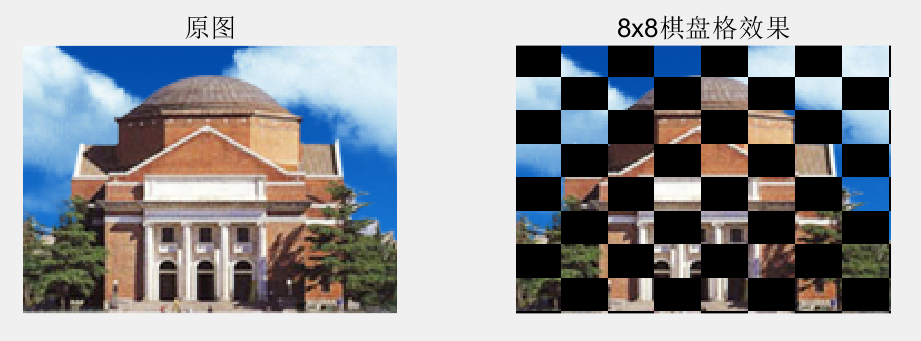
\includegraphics[width=0.7\linewidth]{1_b.png}
    \caption{黑白格}
\end{figure}

\section{图像压缩编码练习题}

\subsection{变换域改变直流分量}

核心代码:
\begin{lstlisting}[language=matlab]
    test_hall=double(hall_gray(1:8,1:8));
    test_hall_1=test_hall-128;

    dct_1=dct2(test_hall_1);
    dct_2=dct2(test_hall);

    dct_2(1,1)=dct_2(1,1)-128*8;

    disp((dct_2-dct_1));
\end{lstlisting}

计算结果为:
\begin{figure}[H]
    \centering
    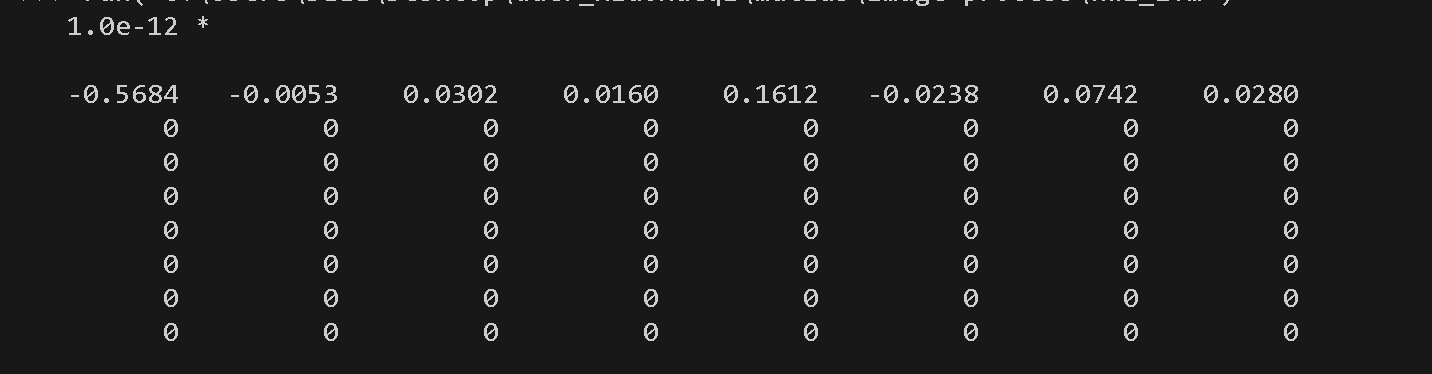
\includegraphics[width=0.7\linewidth]{2_1.png}
    \caption{结果}
\end{figure}

可以看到两个矩阵几乎一样,说明对于一个8*8的灰度值矩阵来说,对原图减128后DCT变换等价于对DCT变换后的矩阵在左上角减去128*8。
原因在于DCT变换有线性性,且常数矩阵的DCT变换只有左上角有非零值。

\subsection{编程实现二维DCT}

核心代码:
\begin{lstlisting}[language = matlab]
    function dct_result = my_dct2(input_matrix)
    [M, ~] = size(input_matrix);
    
    di1 = 1:2:2*M-1;
    di2 = (1:M-1)';
    D = cos(pi/(2*M)*di1.*di2);
    D = sqrt(2/M)*[1/sqrt(2)*ones(1,M); D];
    dct_result = D*input_matrix*D';
end
\end{lstlisting}

\begin{figure}[H]
    \centering
    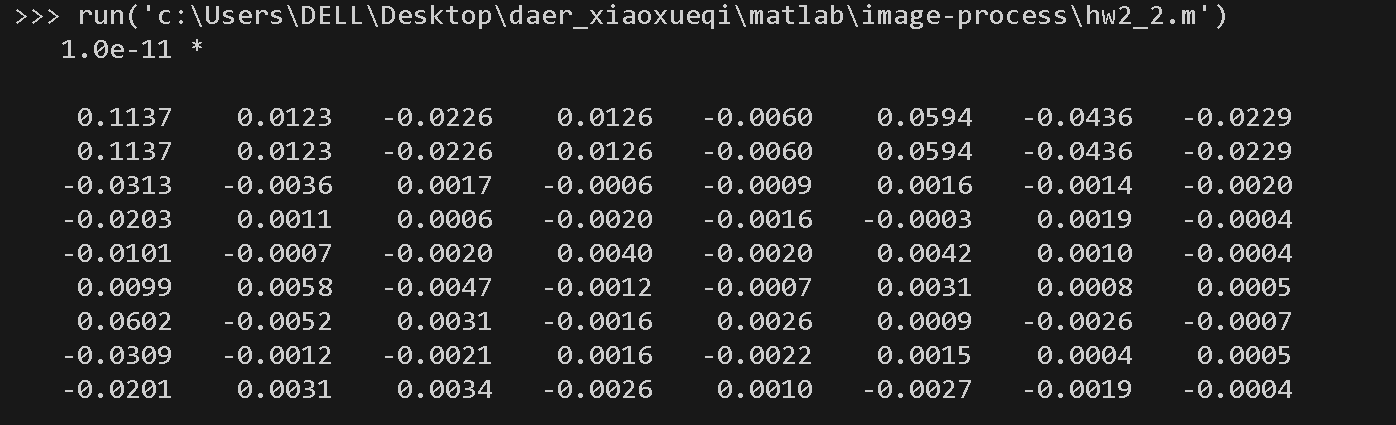
\includegraphics[width=0.7\linewidth]{2_2.png}
    \caption{dct2与自己实现的DCT之差}
\end{figure}

可以看出二者相差很小,说明自己实现的DCT和MATLAB自带的dct2函数是一致的。

\subsection{DCT系数矩阵部分置零}

核心代码:
\begin{lstlisting}[language=matlab]
    % 定义 DCT 处理函数
    dct_left_zero = @(block_struct) dct_left_zero_func(block_struct.data);
    dct_right_zero = @(block_struct) dct_right_zero_func(block_struct.data);
    % 使用 blockproc 处理图像
    C0 = blockproc(initial, [8, 8], @(block_struct) dct2(block_struct.data));
    C1 = blockproc(initial, [8, 8], dct_left_zero);
    C2 = blockproc(initial, [8, 8], dct_right_zero);
    % 反变换并加回 128
    im0 = uint8(blockproc(C0, [8, 8], @(block_struct) idct2(block_struct.data)) + 128);
    im1 = uint8(blockproc(C1, [8, 8], @(block_struct) idct2(block_struct.data)) + 128);
    im2 = uint8(blockproc(C2, [8, 8], @(block_struct) idct2(block_struct.data)) + 128);
    % 左侧四列置零
    function out = dct_left_zero_func(block)
        dct_block = dct2(block);
        dct_block(:, 1:4) = 0;
        out = dct_block;
    end
    % 右侧四列置零
    function out = dct_right_zero_func(block)
        dct_block = dct2(block);
        dct_block(:, 5:8) = 0;
        out = dct_block;
    end
\end{lstlisting}

\begin{figure}[H]
    \centering
    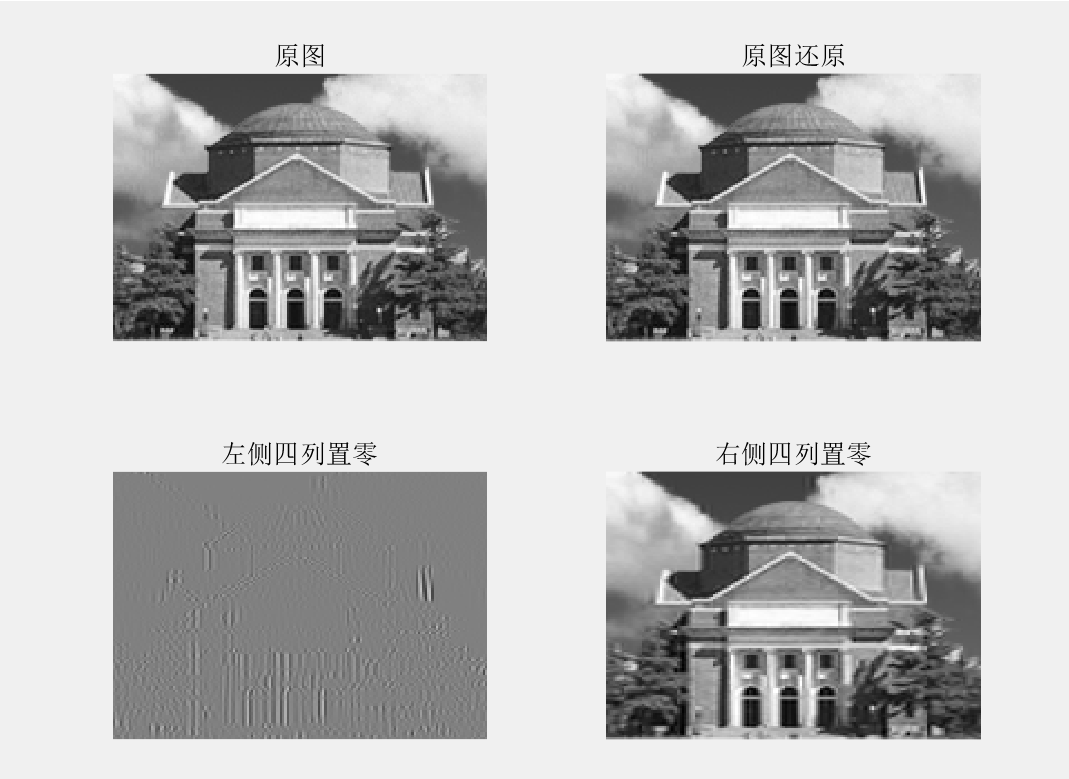
\includegraphics[width=0.7\linewidth]{2_3.png}
    \caption{结果}
\end{figure}

在离散余弦变换的系数矩阵中,左上角的元素代表直流和低频分量,左下角的元素代表纵向变化的高频分量,右上角的元素代表横向变化的高频分量,右
下角的元素代表横向和纵向变化的高频分量。\\
\hspace*{2em}因此将右侧置零对图像的整体影响较小,但是图片在横向上的色彩变化稍显模糊,由于图片本身的高频分量较小,不会对整体造成太大影响;\\
\hspace*{2em}而将左侧四列置零,由于低频分量丢失,原图低频分量本来就比较大,人眼对低频分量更敏感,因此图片质量严重受损。并且由于左下角代表纵向变化的高频分量,因此图像在纵向的变化会降低;\\
\hspace*{2em}综上所述,将左侧四列置零后的图像面目全非,但是能看到一条条的纵向纹理,保留了横向的色彩变化;而将右侧四列置零后的图像质量与原图差别不大,但是在横向上的变化更缓和。

\subsection{系数矩阵转置、旋转}

如图:
\begin{figure}[H]
    \centering
    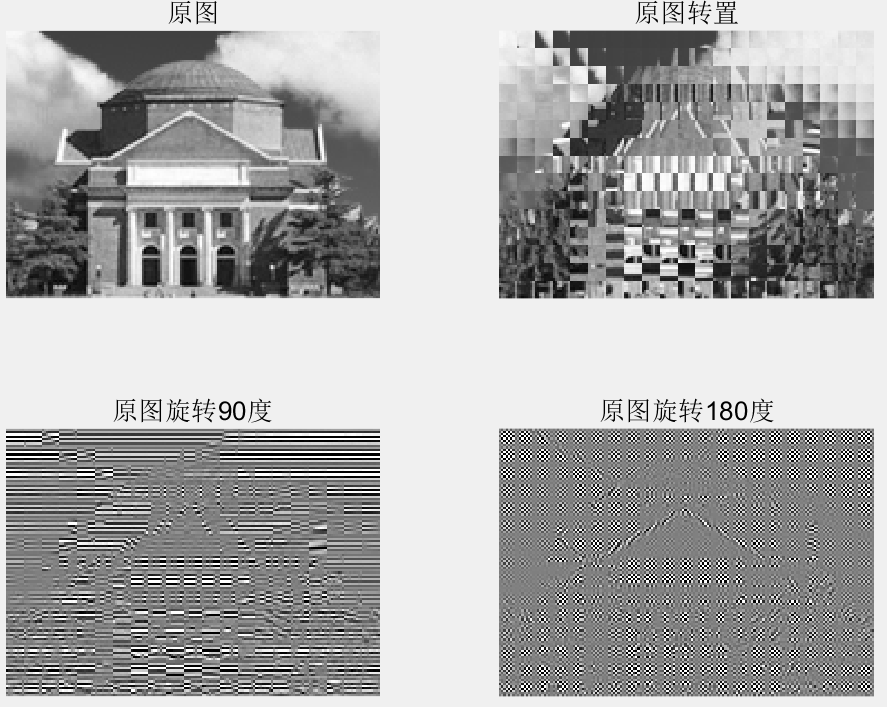
\includegraphics[width=0.7\linewidth]{2_4.png}
    \caption{结果}
\end{figure}

\subsubsection{转置}
我们结合公式:
\begin{equation}
    \mathbf{C} = \mathbf{DPD}^T \qquad \mathbf{P} = \mathbf{D}^T\mathbf{CD}
\end{equation}
\hspace*{2em}两边取转置:
\begin{equation}
    \mathbf{C}^T = \mathbf{DP}^T\mathbf{D}^T \qquad \mathbf{P}^T = \mathbf{D}^T\mathbf{C}^T\mathbf{D}
\end{equation}
\hspace*{2em}可以看到系数矩阵的转置逆变换就是原图像的转置,因此图像会呈现如图所示的效果。

\subsubsection{逆时针旋转90度}
测试的图像有较大的低频分量,旋转90度后,低频分量的系数变为了左下角纵向变化高频分量的系数,得到的图像会在纵向上有较大的变化,呈现明显的横向纹理。
\subsubsection{旋转180度}
旋转180度后,低频分量的系数变为了右下角横向和纵向变化高频分量的系数,得到的图像会在横向和纵向上有较大的变化,呈现明显的黑白交替的网格状纹理。
\subsection{差分系统频率响应}
\begin{equation}
    y(n) = x(n-1) - x(n)
\end{equation}

\begin{figure}[H]
    \centering
    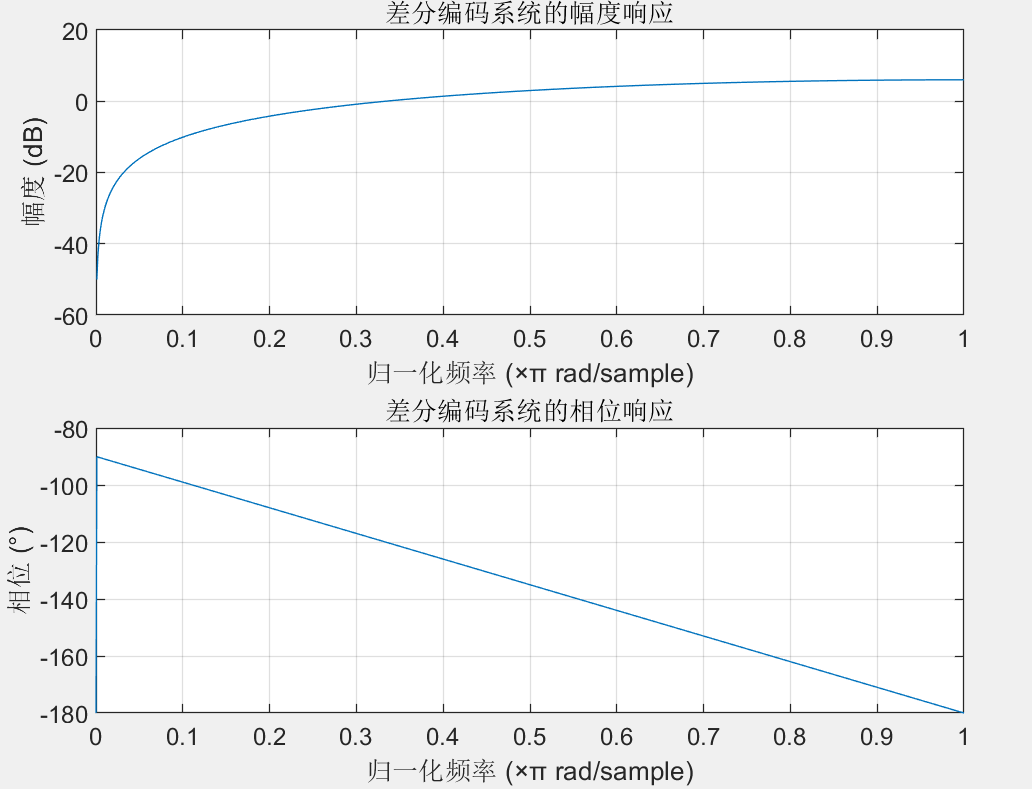
\includegraphics[width=0.7\linewidth]{2_5.png}
    \caption{结果}
\end{figure}
可以看出这是一个高通滤波器,说明需要滤除低频分量,DC系数中的高频分量更多

\subsection{DC 预测误差的取值和 Category 关系}

Category是DC预测误差的二进制表示位数,即:
\begin{equation}
    \text{Category} = \left\lceil \log_2(|Err_{dc}| + 1) \right\rceil
\end{equation}

\subsection{实现zig-zag扫描}

对任意形状矩阵进行zig-zag扫描,同时可以指定扫描方向:

\begin{lstlisting}[language=matlab]
    function zigzag = zig_zag(matrix, direction)
        [m, n] = size(matrix);
        zigzag = zeros(1, m*n);
        [i, j] = deal(1, 1);
        
        for k = 1:m*n
            zigzag(k) = matrix(i, j);
            disp(zigzag(k))
            if direction && (j == 1 || i == m) || ... 
            ~direction && (i == 1 || j == n)
                if direction
                    [i, j] = deal(i + (i < m), j + (i == m));
                else
                    [i, j] = deal(i + (j == n), j + (j < n));
                end
                direction = ~direction;
            else
                [i, j] = deal(i + 2*direction - 1, j - 2*direction + 1);
            end
        end
    end
\end{lstlisting}

\begin{figure}[H]
    \centering
    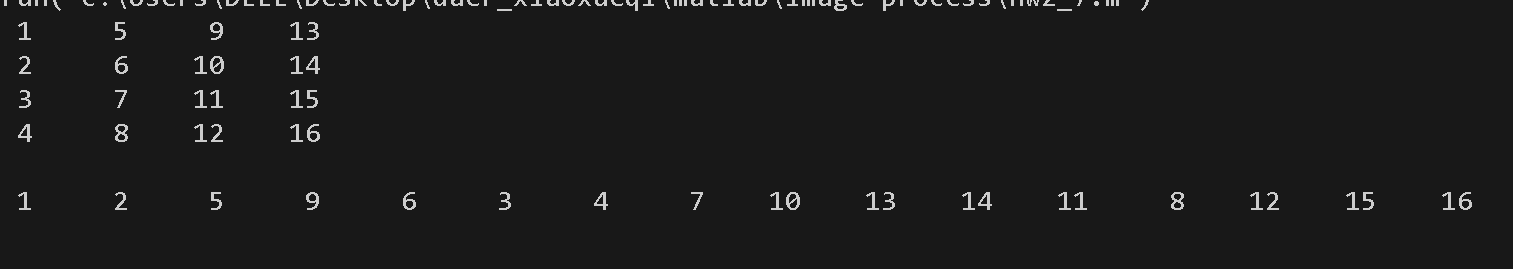
\includegraphics[width=0.7\linewidth]{2_7.png}
    \caption{结果}
\end{figure}

\subsection{图片分块、DCT 和量化}
核心代码:
\begin{lstlisting}[language=matlab]
    initial = double(hall_gray) - 128;
    [height, width] = size(initial);
    w=width/8;
    h=height/8;
    dct_1 = blockproc(initial, [8, 8], @(block_struct) ... 
    dct2(block_struct.data)./QTAB);
    out_matrix = zeros(64, w*h);
    for i = 1:h
        for j = 1:w
            out_matrix(:, (i-1)*w+j) = round(zig_zag(dct_1((i-1)*8+1:i*8, ... 
             (j-1)*8+1:j*8),0));
        end
    end
\end{lstlisting}
结果储存在hw2\_8.csv中

\begin{figure}[H]
    \centering
    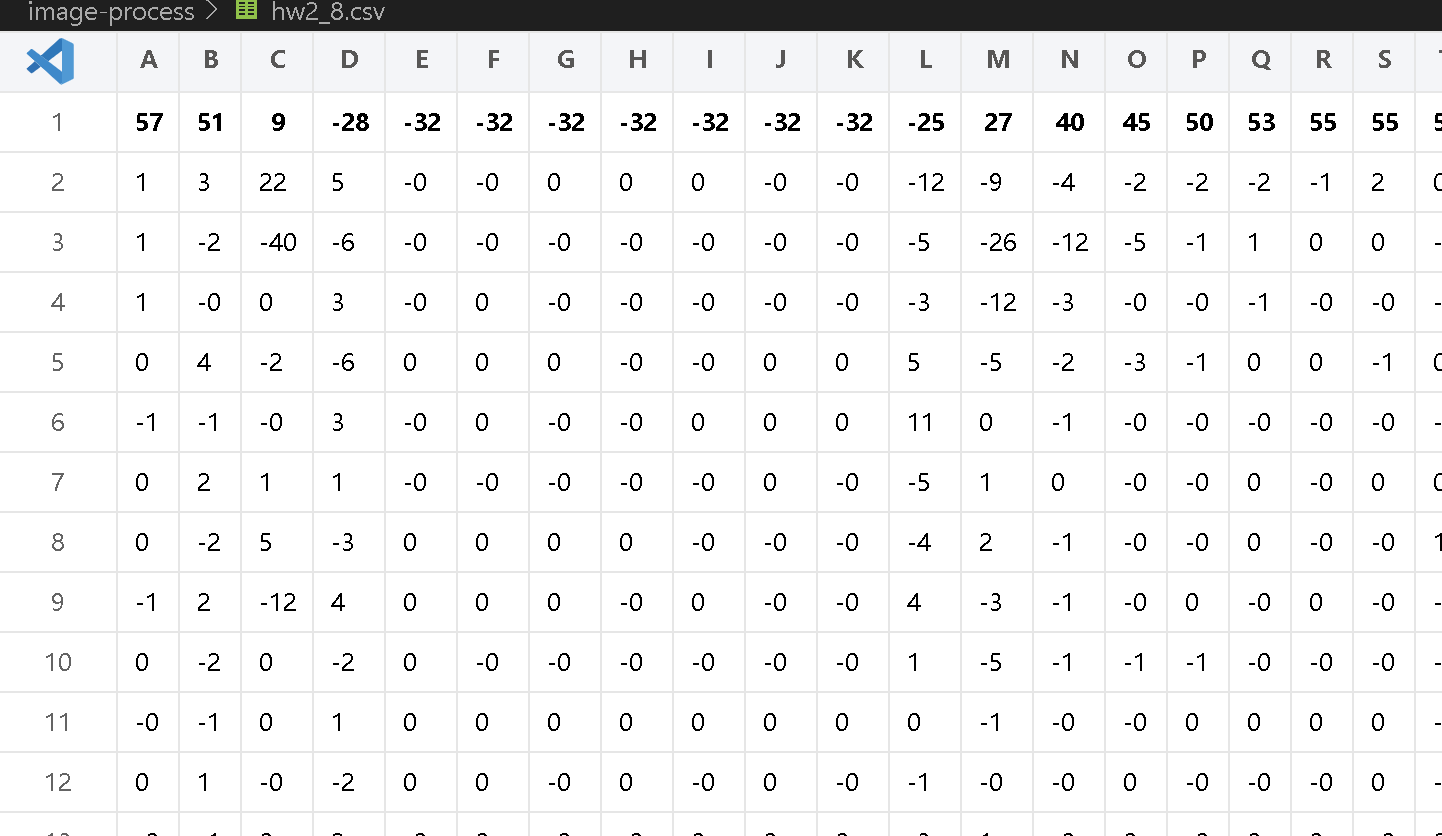
\includegraphics[width=0.7\linewidth]{2_8.png}
    \caption{结果}
\end{figure}

\subsection{JPEG 编码}
dc编码:
\begin{lstlisting}[language=matlab]
    DC_diff = diff(DC);
    DC_diff = [DC(1), -DC_diff];
    %dc_encode
    DC_output = [];
    for i = 1: length(DC_diff)
        j = DC_diff(i);
        category = ceil(log2(abs(j)+1)) + 1;
        len = DCTAB(category, 1);
        huff = DCTAB(category,2:len+1);
        bin = double(dec2bin(abs(j)))-48;
        if j < 0
            bin = ~bin;
        end
        if j == 0
            bin_num = [];
        else
            bin_num = bin;
        end
        DC_output = [DC_output, huff, bin_num];
    end
\end{lstlisting}

ac编码:
\begin{lstlisting}[language=matlab]
    %ac_encode
    AC_output = [];
    for k = 1 : w*h
        AC_k=AC(:,k)';   
        AC_one=[];
        not_zero = find(AC_k);
        if(isempty(not_zero))
            AC_one = [1,0,1,0];
        else
            num_zero = [not_zero(1)-1, diff(not_zero)-1];
            for l = 1:length(num_zero)
                run = num_zero(l);
                if(run > 15)
                    run = run - 16;
                    AC_one = [AC_one, 1, 1, 1, 1, 1, 1, 1, 1, 0, 0, 1];
                end
                amplitude = AC_k(not_zero(l));
                size_ = ceil(log2(abs(amplitude)+1));
                idx = find(ACTAB(:,1)==run & ACTAB(:,2)==size_);
                len = ACTAB(idx,3);
                huff = ACTAB(idx,4:len+3);
                bin = double(dec2bin(abs(amplitude)))-48;
                if(amplitude < 0)
                    bin = ~bin;
                end
                if amplitude == 0
                    bin_num = [];
                else
                    bin_num = bin;
                end
                AC_one = [AC_one, huff, bin_num];
            end
            AC_one = [AC_one, 1,0,1,0];
        end
        AC_output = [AC_output, AC_one];
    end
\end{lstlisting}

保存结果:
\begin{lstlisting}[language=matlab]
    save jpegcodes.mat DC_output AC_output height width
\end{lstlisting}

\subsection{计算压缩比}

\begin{figure}[H]
    \centering
    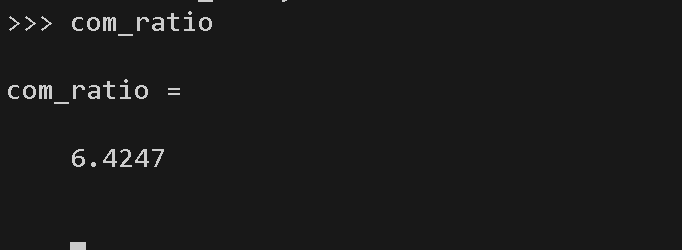
\includegraphics[width=0.7\linewidth]{2_10.png}
    \caption{压缩比}
\end{figure}

压缩比约为6.4247

\subsection{JPEG 解码}

dc解码:
\begin{lstlisting}[language=matlab]
    DC_re = zeros(1,block_num);
    i=1;
    idx=1;
    while i <= length(DC_output)
        for j = 1:size(DCTAB,1)
            if DCTAB(j,2:DCTAB(j,1)+1) == DC_output(i:i+DCTAB(j,1)-1)
                category = j-1;
                i = i+DCTAB(j,1);
                if(category == 0)
                    DC_re(idx) = 0;
                    idx=idx+1;
                else
                    magnitude = DC_output(i:i+category-1);
                    if(magnitude(1) == 0)
                        DC_re(idx) = -bin2dec(char(~magnitude+48));
                        idx=idx+1;
                    else
                        DC_re(idx) = bin2dec(char(magnitude+48));
                        idx=idx+1;
                    end
                end
                i = i+category;
                break;
            end
        end
    end
    for k = 2: block_num
        DC_re(k) = DC_re(k-1)-DC_re(k);
    end
\end{lstlisting}

ac解码:

\begin{lstlisting}[language=matlab]
    AC_re = zeros(block_num,63);
    idx_1=1;
    idx_2=1;
    idx_3=1;
    ZRL = [1,1,1,1,1,1,1,1,0,0,1];
    EOB = [1,0,1,0];
    while idx_1 <= length(AC_output)
        if EOB == AC_output(idx_1:idx_1+3)
            idx_1 = idx_1+4;
            idx_2 = idx_2+1;
            idx_3 = 1;
        elseif ZRL == AC_output(idx_1:idx_1+10) & idx_1 <=... 
         length(AC_output)-10
            AC_re(idx_2,idx_3:idx_3+15) = 0;
            idx_1 = idx_1+11;
            idx_3 = idx_3+16;
        else
            for j = 1:size(ACTAB,1)
                if idx_1 + ACTAB(j,3) -1 <= length(AC_output) & ... 
                ACTAB(j,4:ACTAB(j,3)+3)==AC_output(idx_1:idx_1+ACTAB(j,3)-1) 
                    %idx_3 = idx_3+ACTAB(j,1);
                    idx_1 = idx_1+ACTAB(j,3);
                    AC_re(idx_2, idx_3:idx_3+ACTAB(j,1)-1) = 0;
                    idx_3 = idx_3+ACTAB(j,1);
                    amplitude = AC_output(idx_1:idx_1+ACTAB(j,2)-1);
                    if amplitude(1) == 0
                        AC_re(idx_2,idx_3) = -bin2dec(char(~amplitude+48));
                        idx_3 = idx_3+1;
                    else
                        AC_re(idx_2,idx_3) = bin2dec(char(amplitude+48));
                        idx_3 = idx_3+1;
                    end
                    idx_1 = idx_1+ACTAB(j,2);
                    break
                end
            end
        end
    end
    AC_re =AC_re';
\end{lstlisting}

重新排列、反zig-zag、反dct2:

\begin{lstlisting}[language=matlab]
    im_re = cat(1, DC_re, AC_re);
    w=width/8;
    h=height/8;
    im_block = zeros(1,64);
    index = reshape(1:64,8,8)';
    indxe_1 = zig_zag(index,1);
    for i = 1:h
        for j = 1:w
            im_block(indxe_1) = im_re(:,(i-1)*w+j);
            im_block = reshape(im_block,8,8);
            im_block = idct2(im_block.*QTAB);
            re_image((i-1)*8+1:i*8,(j-1)*8+1:j*8) = im_block;
        end
    end
    re_image = uint8(re_image+128);
\end{lstlisting}

恢复的图像与原图如下:

\begin{figure}[H]
    \centering
    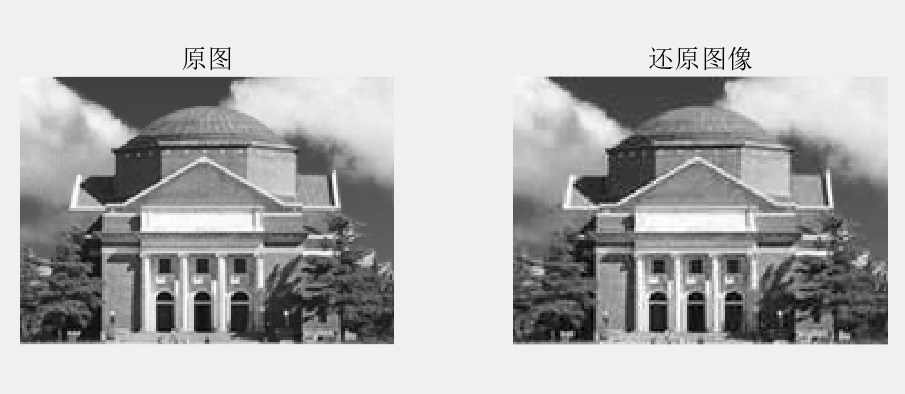
\includegraphics[width=0.7\linewidth]{2_11_2.png}
    \caption{原图与还原图像}
\end{figure}

\begin{figure}[H]
    \centering
    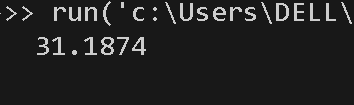
\includegraphics[width=0.7\linewidth]{2_11_1.png}
    \caption{PSNR}
\end{figure}

从主观上来说,还原的图像与原图几乎一致,说明JPEG编解码的效果很好;从客观上来说,PSNR为31.1874dB,说明还原的图像与原图的差别很小。

\subsection{减半量化步长}

核心代码:
\begin{lstlisting}[language=matlab]
    QTAB = QTAB / 2;
    [DC_output, AC_output, width, height] = encode(hall_gray, QTAB, DCTAB, ACTAB);
    com_ratio = width * height * 8 / (length(DC_output) + length(AC_output));
    disp(com_ratio);
    re_image = decode(DC_output, AC_output, width, height, QTAB, DCTAB, ACTAB);
\end{lstlisting}

\begin{figure}[H]
    \centering
    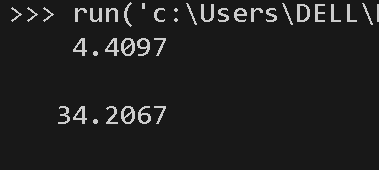
\includegraphics[width=0.7\linewidth]{2_12_1.png}
    \caption{压缩比和PSNR}
\end{figure}

\begin{figure}[H]
    \centering
    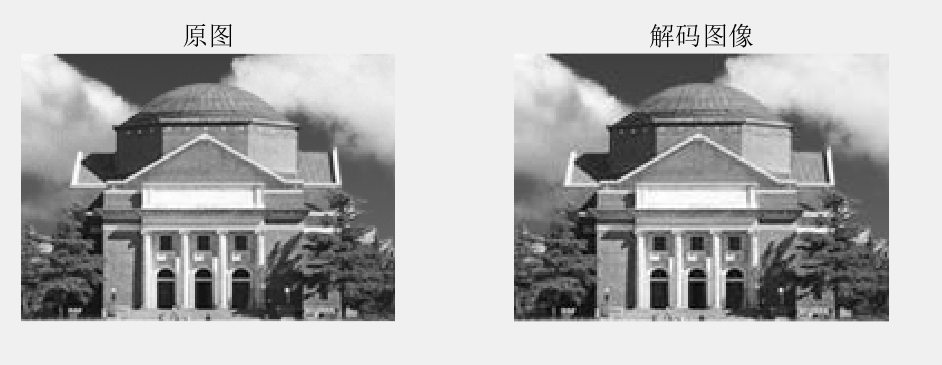
\includegraphics[width=0.7\linewidth]{2_12_2.png}
    \caption{量化步长减小一半}
\end{figure}

可以看到压缩比变为4.4097,PSNR变为34.2067dB,压缩比减小,损失的信息更少,因此PSNR更高,图像质量更好。

\subsection{处理雪花图像}
\begin{figure}[H]
    \centering
    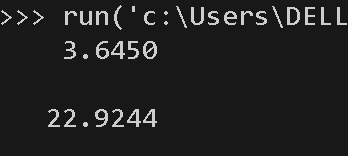
\includegraphics[width=0.6\linewidth]{2_13_1.png}
    \caption{压缩比和PSNR}
\end{figure}

\begin{figure}[H]
    \centering
    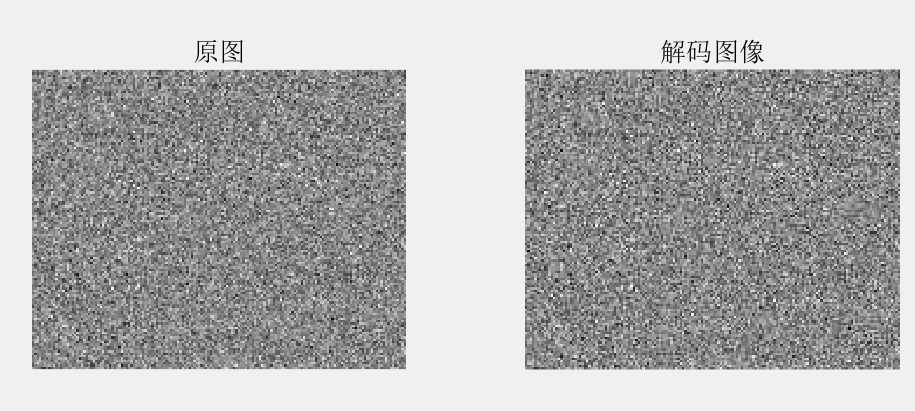
\includegraphics[width=0.7\linewidth]{2_13_2.png}
    \caption{雪花图像原图及还原图}
\end{figure}

压缩比为3.6450,PSNR为22.9244dB,压缩比比之前更低,PSNR也更低,原因可能是雪花图像的随机性较强,图片的高频分量更大,不容易被量化为0,压缩比较低;
由于高频分量被量化,使得以高频分量为主的雪花图损失较多信息,PSNR较低。

\section{信息隐藏练习题}
\subsection{空域隐藏信息}

\begin{lstlisting}[language=matlab]
    info_size = width * height ;
    info = dec2bin(randi([0, 1], info_size, 1));
    hall_bin = dec2bin(hall_gray);
    hall_bin(:,8)=info;
    hall_image = bin2dec(hall_bin);
    hall_image_1 = reshape(hall_image, height, width);

    [DC_output, AC_output, width, height] = ... 
     encode(hall_image_1, QTAB, DCTAB, ACTAB);
    hall_image_2 = decode(DC_output, AC_output, width, height, QTAB, DCTAB, ACTAB);

    hall_bin_2 = dec2bin(hall_image_2);
    info_2 = hall_bin_2(:,8);
    accuracy = sum(info == info_2) / info_size;
\end{lstlisting}

测试10次,得到结果:
\begin{figure}[H]
    \centering
    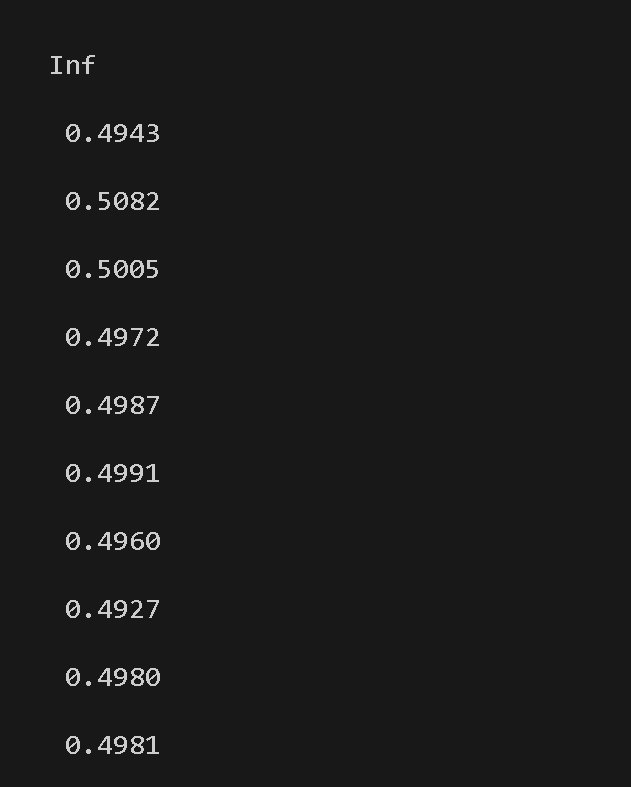
\includegraphics[width=0.4\linewidth]{3_1_2.png}
    \caption{准确率}
\end{figure}
看到准确率在0.5左右,而我们的信息都是0或1,说明信息几乎没有被保留;
\hspace*{2em}原因在于我们在空域隐藏信息时只修改了最低位,而量化过程会将这部分信息丢失,反量化后无法获取原来的信息,因此空域隐藏抗JPEG编码能力很低

\subsection{变换域隐藏信息}
\subsubsection{信息隐藏在每个系数的最低位}

\begin{lstlisting}[language=matlab]
    info_in = dec2bin(randi([0,1],width*height,1));
    out_matrix_bin = dec2bin(out_matrix);
    out_matrix_bin(:,8) = info_in;
    out_matrix_2 = signed_bin2dec(out_matrix_bin);
    out_matrix_3 = reshape(out_matrix_2, 64 , w*h);
\end{lstlisting}
\begin{figure}[H]
    \centering
    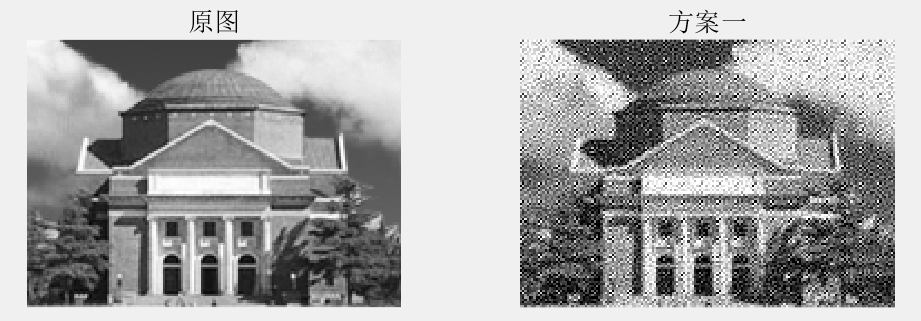
\includegraphics[width=0.8\linewidth]{3_2_1.png}
    \caption{原图及复原图}
\end{figure}

\begin{figure}[H]
    \centering
    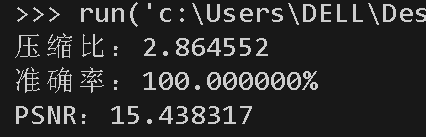
\includegraphics[width=0.6\linewidth]{3_2_1_0.png}
    \caption{结果}
\end{figure}

信息恢复准确率为100\%,压缩比为2.8646,PSNR为15.4383dB

\subsubsection{信息隐藏在部分系数的最低位}

首先设置好比例ratio,代表对每ratio个量化后的系数进行信息位的替换,这里设置为2\\
\hspace*{2em}\textbf{采用两种方案进行实现比较:}
\subsubsubsection{按顺序,每两个系数替换一个信息位}

\hspace*{2em}实现代码:
\begin{lstlisting}[language=matlab]
    ratio = 2
    info_num = width * height / ratio ;
    info_in = dec2bin(randi([0,1],info_num,1));

    out_matrix_bin = dec2bin(out_matrix);
    for i = 1:info_num
        out_matrix_bin(i*ratio,8) = info_in(i);
    end
\end{lstlisting}

效果如图:
\begin{figure}[H]
    \centering
    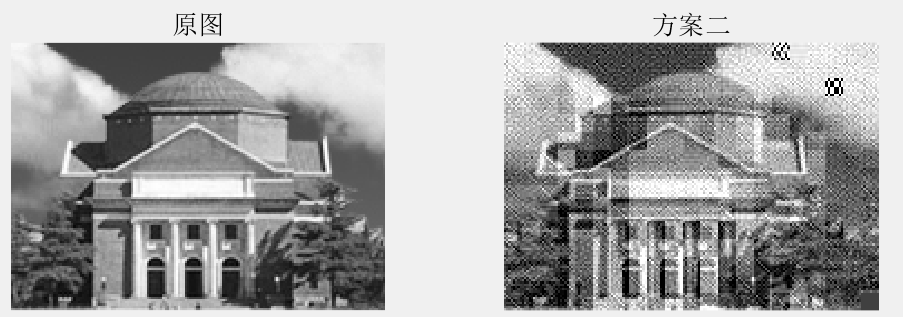
\includegraphics[width=0.8\linewidth]{3_2_2_1.png}
    \caption{原图及复原图}
\end{figure}

\begin{figure}[H]
    \centering
    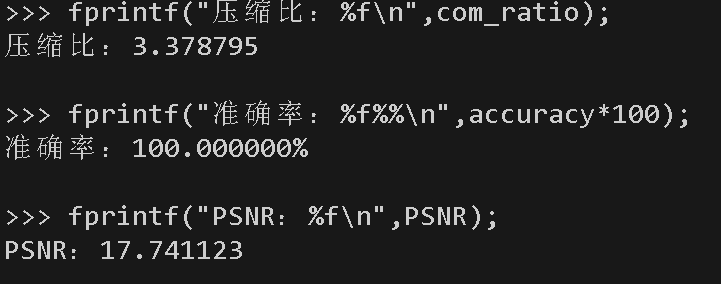
\includegraphics[width=0.6\linewidth]{3_2_2_1_0.png}
    \caption{结果}
\end{figure}

信息恢复准确率为100\%,压缩比为3.3788,PSNR为17.7411dB\\
\subsubsubsection{挑选量化系数矩阵中较小的一半,在对应的位置处替换信息位}

实现代码:
\begin{lstlisting}[language=matlab]
    ratio = 2
    indices = find_smaller_ones(QTAB, ratio);
    info_num = width * height / ratio ;
    info_in = dec2bin(randi([0,1],info_num,1));

    out_matrix_bin = dec2bin(out_matrix);
    for i = 1:w*h
        for j = 1: ceil(64/ratio)
            out_matrix_bin(64*(i-1)+indices(j),8) = info_in((i-1)*64/ratio+j);
        end
    end
\end{lstlisting}

自定义函数find\_smaller\_ones:
\begin{lstlisting}[language=matlab]
    function indices = find_smaller_ones(matrix, ratio)
        flattened = zig_zag(matrix, 0);
        num_to_select = ceil(numel(flattened) / ratio);
        [~, sorted_indices] = sort(flattened);
        indices = sorted_indices(1:num_to_select);
    end
\end{lstlisting}

效果如图:
\begin{figure}[H]
    \centering
    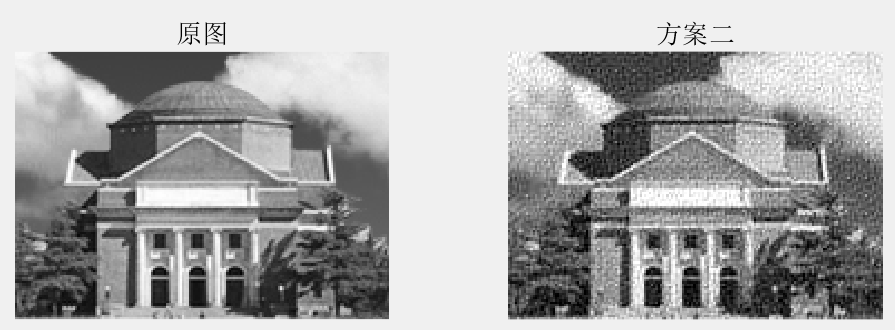
\includegraphics[width=0.8\linewidth]{3_2_2_2.png}
    \caption{原图及复原图}
\end{figure}

\begin{figure}[H]
    \centering
    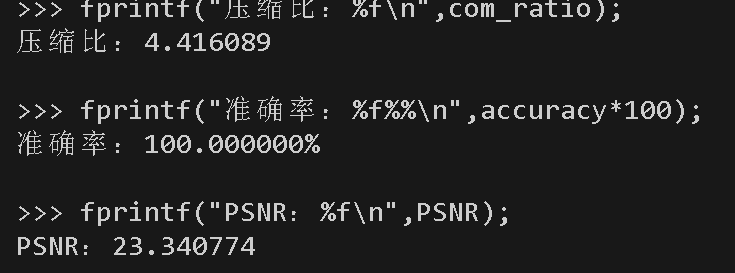
\includegraphics[width=0.6\linewidth]{3_2_2_2_0.png}
    \caption{结果}
\end{figure}

信息恢复准确率为100\%,压缩比为4.4161,PSNR为23.3408dB\\

可以看到隐藏同等信息量的情况下,方案二的压缩比和PSNR都更优秀,说明方案二更适合信息隐藏

\subsubsection{信息隐藏在最后一个非零位之后}

实现代码:
\begin{lstlisting}[language=matlab]
    info_num = w * h ;
    info_in = double(randi([0,1],info_num,1));
    info_in = info_in * 2 - 1;

    out_matrix_3 = out_matrix;
    for i = 1:info_num
        not_zero = find(out_matrix_3(:,i));
        if not_zero(end) == 64
            out_matrix_3(64,i) = info_in(i);
        else
            out_matrix_3(not_zero(end)+1,i) = info_in(i);
        end
    end
\end{lstlisting}

效果如图:
\begin{figure}[H]
    \centering
    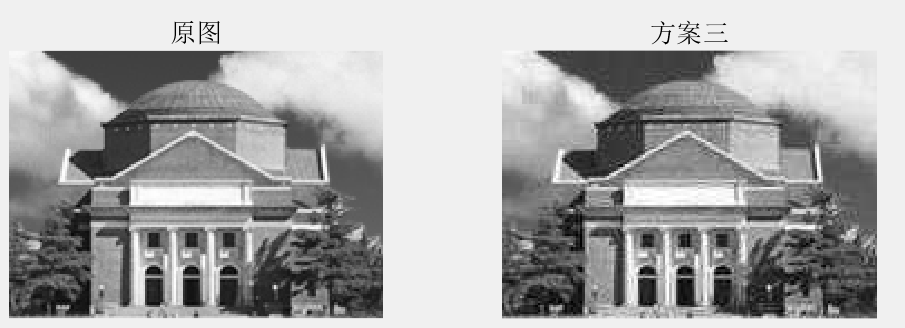
\includegraphics[width=0.8\linewidth]{3_2_3_1.png}
    \caption{原图及复原图}
\end{figure}

\begin{figure}[H]
    \centering
    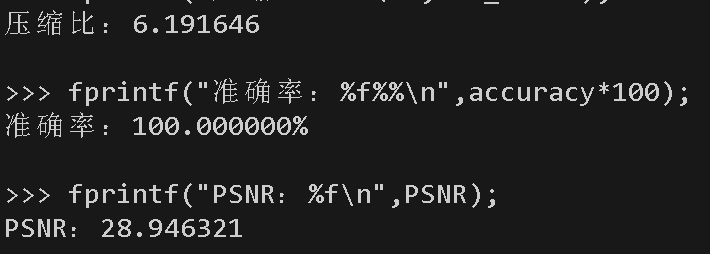
\includegraphics[width=0.6\linewidth]{3_2_3_1_0.png}
    \caption{结果}
\end{figure}

信息恢复准确率为100\%,压缩比为6.1916,PSNR为28.9463dB\\

这里我们继续应用方案二,保证隐藏信息量相同(设置ratio为64)的情况下比较效果:
\begin{figure}[H]
    \centering
    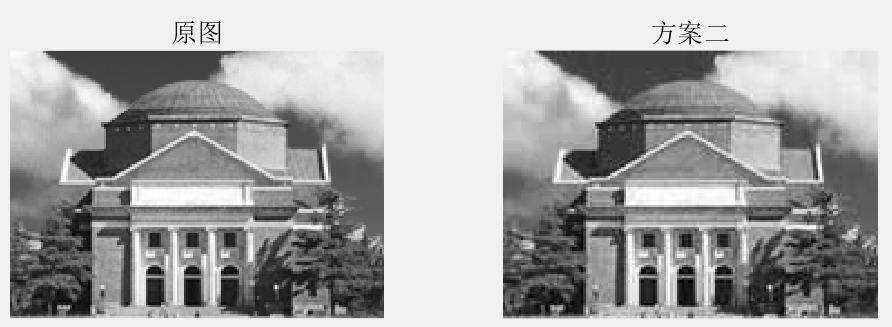
\includegraphics[width=0.8\linewidth]{3_2_3_2.png}
    \caption{原图及复原图}
\end{figure}

\begin{figure}[H]
    \centering
    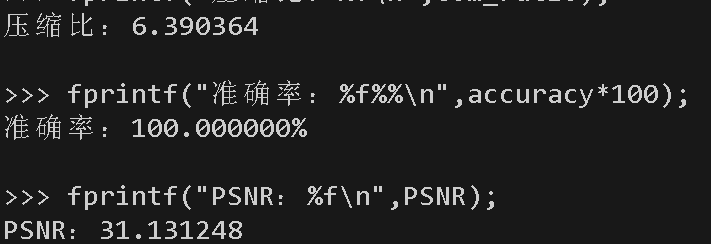
\includegraphics[width=0.6\linewidth]{3_2_3_2_0.png}
    \caption{结果}
\end{figure}

信息恢复准确率为100\%,压缩比为6.3904,PSNR为31.1312dB\\

\hspace*{2em}压缩比和PSNR均大于方案三,说明此方案更适合信息隐藏

\subsubsection{总结比较}

效果对比如下:
\begin{table}[H]
    \centering
    \begin{tabular}{|c|c|c|c|}
    \hline
    方案 & 压缩比 & PSNR/dB & 准确率/\%  \\
    \hline
    替换所有系数 & 2.8646 & 15.4383 & 100 \\
    \hline
    顺序每两个系数替换一个信息位 & 3.3788 & 17.7411 & 100 \\
    \hline
    选取较小的一半系数替换信息位 & 4.4161 & 23.3408 & 100\\
    \hline
    信息隐藏在最后一个非零位之后 & 6.1916 & 28.9463 & 100\\
    \hline
    选取最小的系数替换信息位 & 6.3904 & 31.1312 & 100 \\
    \hline
    \end{tabular}
\end{table}

可以看到,第一种方案由于隐藏的信息量最大,所以压缩比和PSNR均比较低;选取QTAB矩阵中较小的参数对应的位置的系数进行替换效果最好,因为QTAB矩阵中参数较小的位置对应的是较小的系数,将信息隐藏在这里能够较小对图像质量的影响

\section{人脸识别练习题}
\subsection{训练人脸标准v }
\subsubsection{是否需要调整大小}
我们只需要获取各种颜色占据图片的比例,因此无需调整图片大小
\subsubsection{训练}
生成v的代码如下:
\begin{lstlisting}[language=matlab]
    function v = generate_v(image_in, L)
        v = zeros(1, 2^(3 * L));
        [h, w, ~] = size(image_in);
        image_re = reshape(image_in, h * w, 3);
        for i = 1 : h*w
            index = floor(double(image_re(i,1))/(2^(8-L))) * 2^(2*L) + ... 
            floor(double(image_re(i,2))/(2^(8-L))) * 2^L + ... 
            floor(double(image_re(i,3))/(2^(8-L))) + 1;
            v(index) = v(index) + 1;
        end
        v = v / (h * w);
    end
\end{lstlisting}

完整代码:
\begin{lstlisting}[language=matlab]
    v_all = struct();
    for L = 3 : 5
        v = zeros(1,2^(3*L));
        for i = 1 : 33
            image_path = sprintf('resources/Faces/%d.bmp',i);
            v = v + generate_v(imread(image_path), L);
        end
        v = v / 33;
        subplot(3,1,L-2);
        plot(v);
        title(sprintf('L = %d', L));
        v_all.(sprintf('v_L%d', L)) = v;
    end
    % 储存所有的 v
    save('all_v.mat', '-struct', 'v_all');
\end{lstlisting}

绘制L:
\begin{figure}[H]
    \centering
    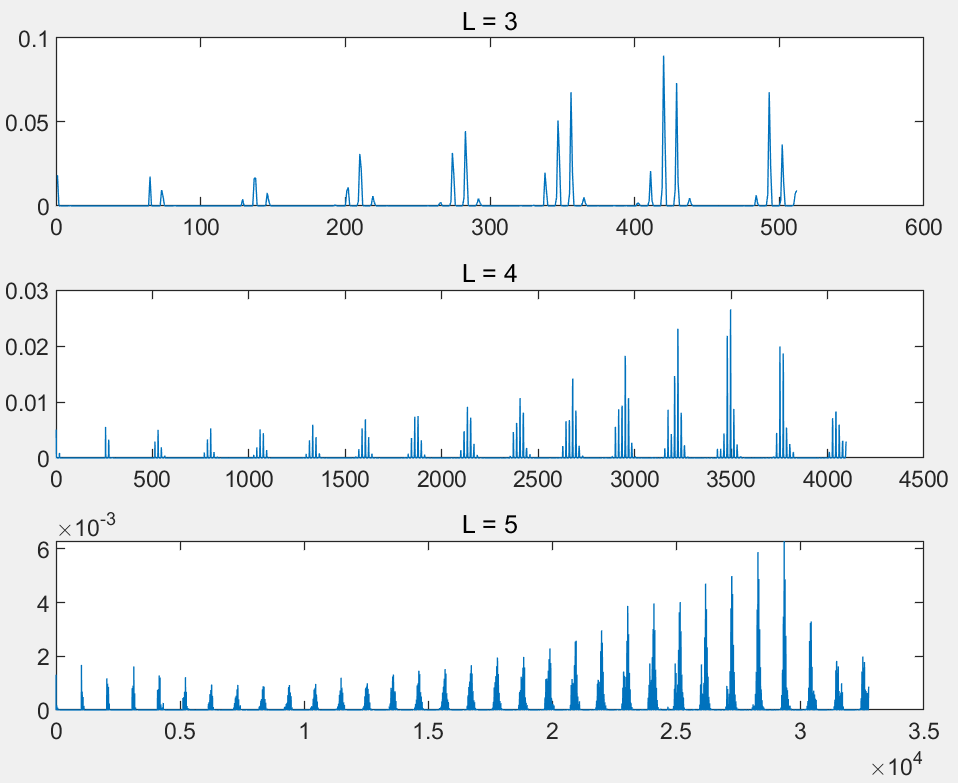
\includegraphics[width=0.7\linewidth]{4_1.png}
    \caption{v}
\end{figure}

可以看到,L越大,不同区域之间的区分度越大;L越小,不同区域之间的区分度越小。\\
\hspace*{2em} L较低的向量可以看作是L较高的向量的近似,向量的值相当于L较高向量对应位置周围值的求和
\subsection{人脸识别}
说明:此部分的思路参考了9字班学长的\href{https://github.com/Timothy-Liuxf/THUEE_MATLAB/tree/master/image}{方法},但是在原有方法上有较大优化\\
\hspace*{2em}初版算法思路:设置好步长和窗口大小,在测试图像上滑动窗口,计算每一个窗口与人脸标准的相近程度,小于阈值则认为是人脸,如此得到小矩形的位置,然后将小矩形合并得到大矩形后绘制红色方框。
为了提高算法的普适性,我选择了一张识别难度较大的图像:

\begin{figure}[H]
    \centering
    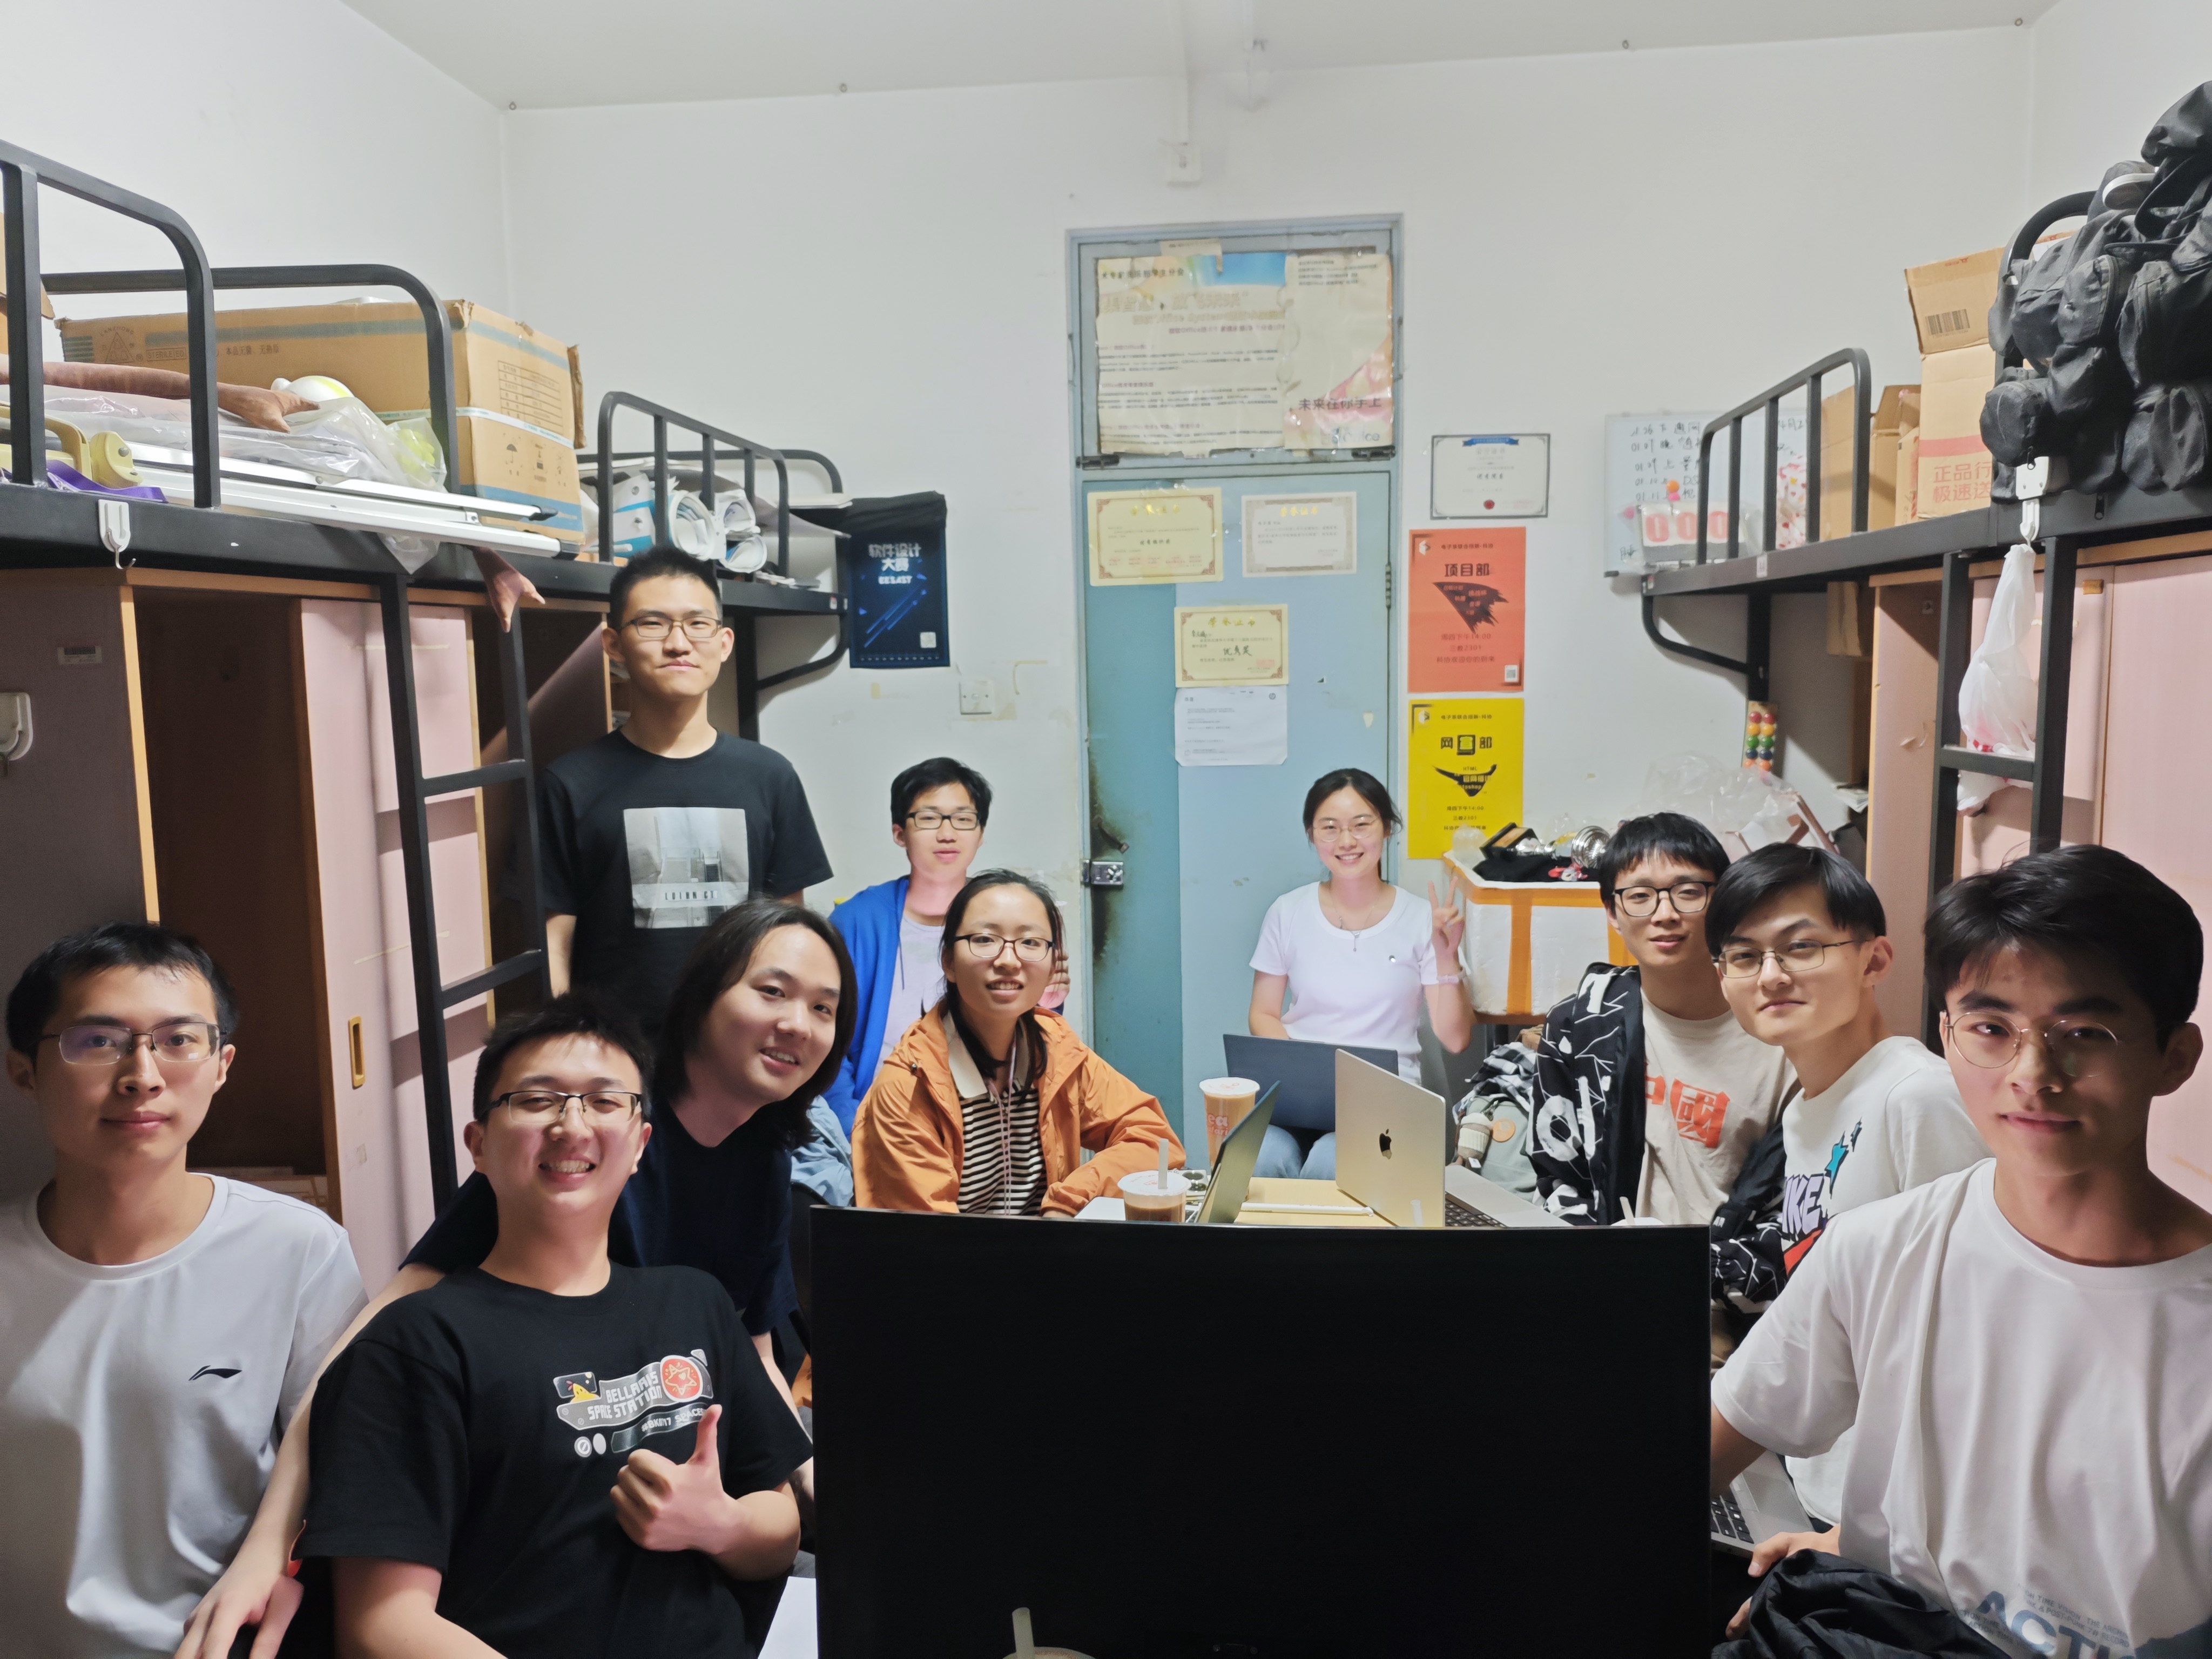
\includegraphics[width=0.6\linewidth]{web_group.jpg}
    \caption{软件部网站组}
\end{figure}

主要代码:\\
\hspace*{2em}首先计算每个单元的v值,与给定v进行比较
\begin{lstlisting}[language=matlab]
    for h = 1 : h_num
        for w = 1 : w_num
            h_start = (h-1) * h_step;
            w_start = (w-1) * w_step;
            test_img = img(h_start + 1 : h_start + h_unit, ... 
            w_start + 1 : w_start + w_unit, :);
            test_v = generate_v(test_img, L);
            diff = 1 - sum(sqrt(test_v) .* sqrt(v));
            if diff < threshold
                unit_count = unit_count + 1;
                unit_top(unit_count) = h;
                unit_left(unit_count) = w;
            end
        end
    end
\end{lstlisting}

然后对二维图像进行连通区域标记并计算每个区域的边界

\begin{lstlisting}[language=matlab]
    % 对二值图像进行连通区域标记
    [labs, n] = bwlabel(img_detect);
    min_left = zeros(n, 1) + w_num;
    min_top = zeros(n, 1) + h_num;
    max_right = zeros(n, 1);
    max_bottom = zeros(n, 1);
    
    % 计算每个连通区域的边界
    for i = 1 : unit_count
        lab = labs(unit_top(i), unit_left(i));
        min_left(lab) = min(min_left(lab), unit_left(i));
        min_top(lab) = min(min_top(lab), unit_top(i));
        max_right(lab) = max(max_right(lab), unit_left(i)+w_multiple-1);
        max_bottom(lab) = max(max_bottom(lab), unit_top(i)+h_multiple-1);
    end
\end{lstlisting}

最后绘制矩形:
\begin{lstlisting}
    top_start = (min_top(i) - 1) * h_step + 1;
    bottom_end = max_bottom(i) * h_step;
    left_start = (min_left(i) - 1) * w_step + 1;
    right_end = max_right(i) * w_step;
    draw_rectangle( top_start : bottom_end, ... 
    left_start : left_start + line_width) = true;
    draw_rectangle( top_start : top_start + line_width, ... 
     left_start: right_end) = true;
    draw_rectangle( top_start: bottom_end, ... 
    max(1, right_end - line_width) : right_end) = true;
    draw_rectangle(max(1, bottom_end - line_width) : bottom_end, ... 
    left_start : right_end) = true;
    
    % 绘制红色边框的矩形
    draw = cat(3, draw_rectangle, false(size(draw_rectangle)), ... 
    false(zeros(size(draw_rectangle))));
    img_in(draw) = uint8(255);
    img_out = img_in;
\end{lstlisting}

图像中的人脸大小不一,明暗不一,还有人体的其他部位干扰(手、胳膊),初版算法的识别效果如下:

\begin{figure}[H]
    \centering
    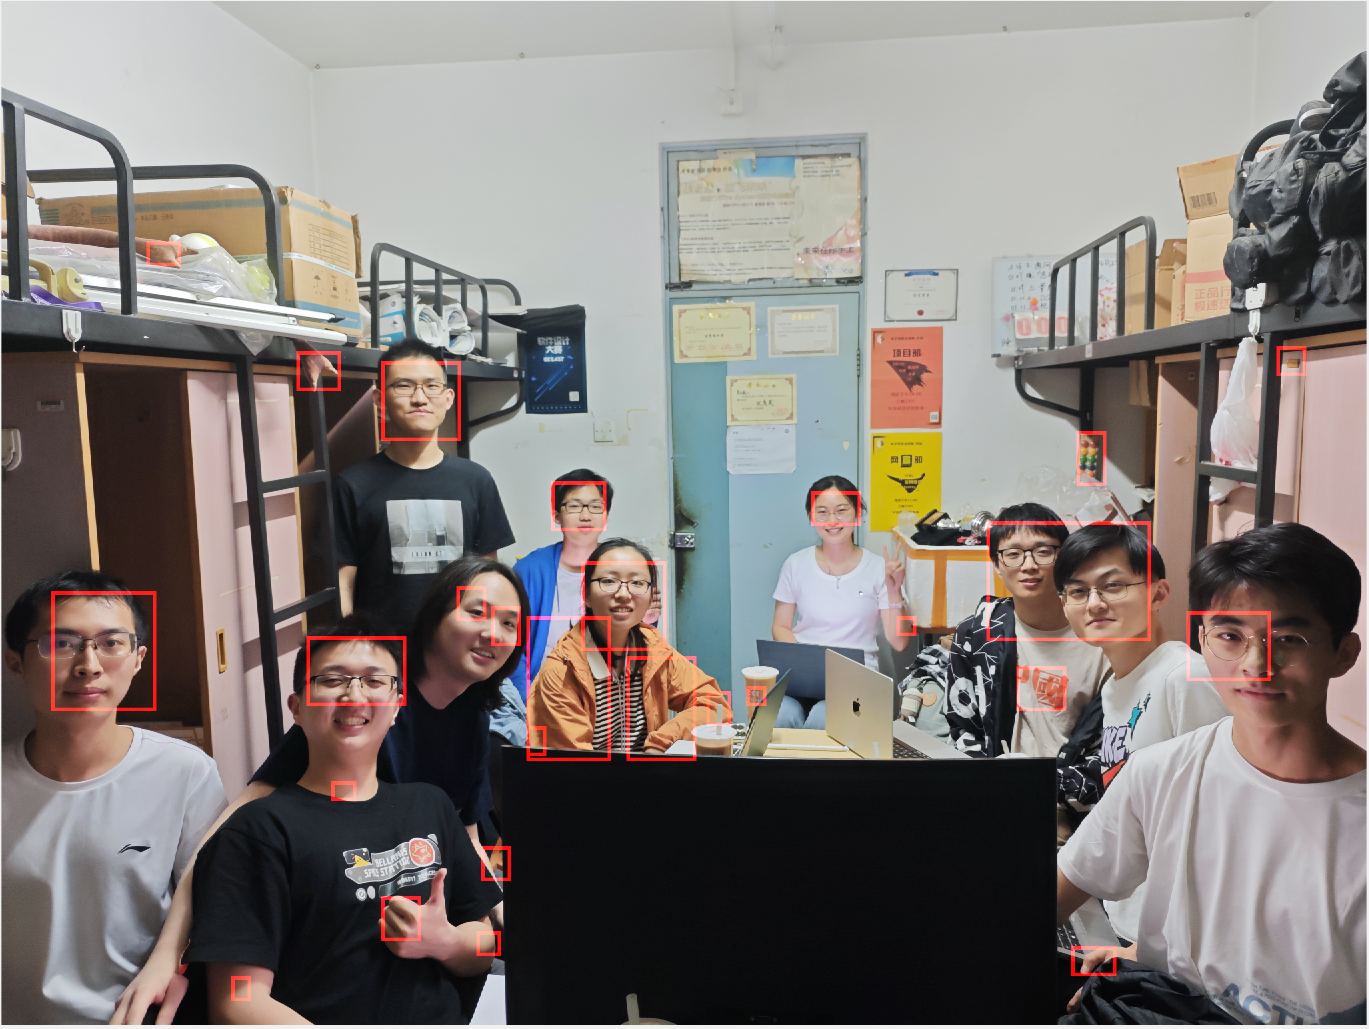
\includegraphics[width=0.6\linewidth]{shibie1.png}
    \caption{识别1}
\end{figure}

可以看到识别效果不好,即使调整了多次参数依然有以下问题:\\
\hspace*{2em}1. 始终有一些小矩形 \\
\hspace*{2em}2. 多个人脸合并到了一起\\
\hspace*{2em}3. 部分大矩形没有完全将人脸框住\\
\hspace*{2em}4. 矩形之间有重叠\\
\hspace*{2em}下面进行优化

算法优化历程:

\subsubsection{优化1:过滤小矩形}
过滤掉大小小于一定阈值以及长宽比大于一定阈值的矩形

代码:
\begin{lstlisting}
    % 去除过小或者太狭长的区域
    flags = ones(n, 1);
    for i = 1 : n
        r_w = double(max_right(i) - min_left(i) +1);
        r_h = double(max_bottom(i) - min_top(i) +1);
        if ((r_w < min_len) && (r_h < min_len)) ... 
        || r_w / r_h >= 1.9 || r_h / r_w >= 1.9
            flags(i) = 0;
        end
    end
\end{lstlisting}

\begin{figure}[H]
    \centering
    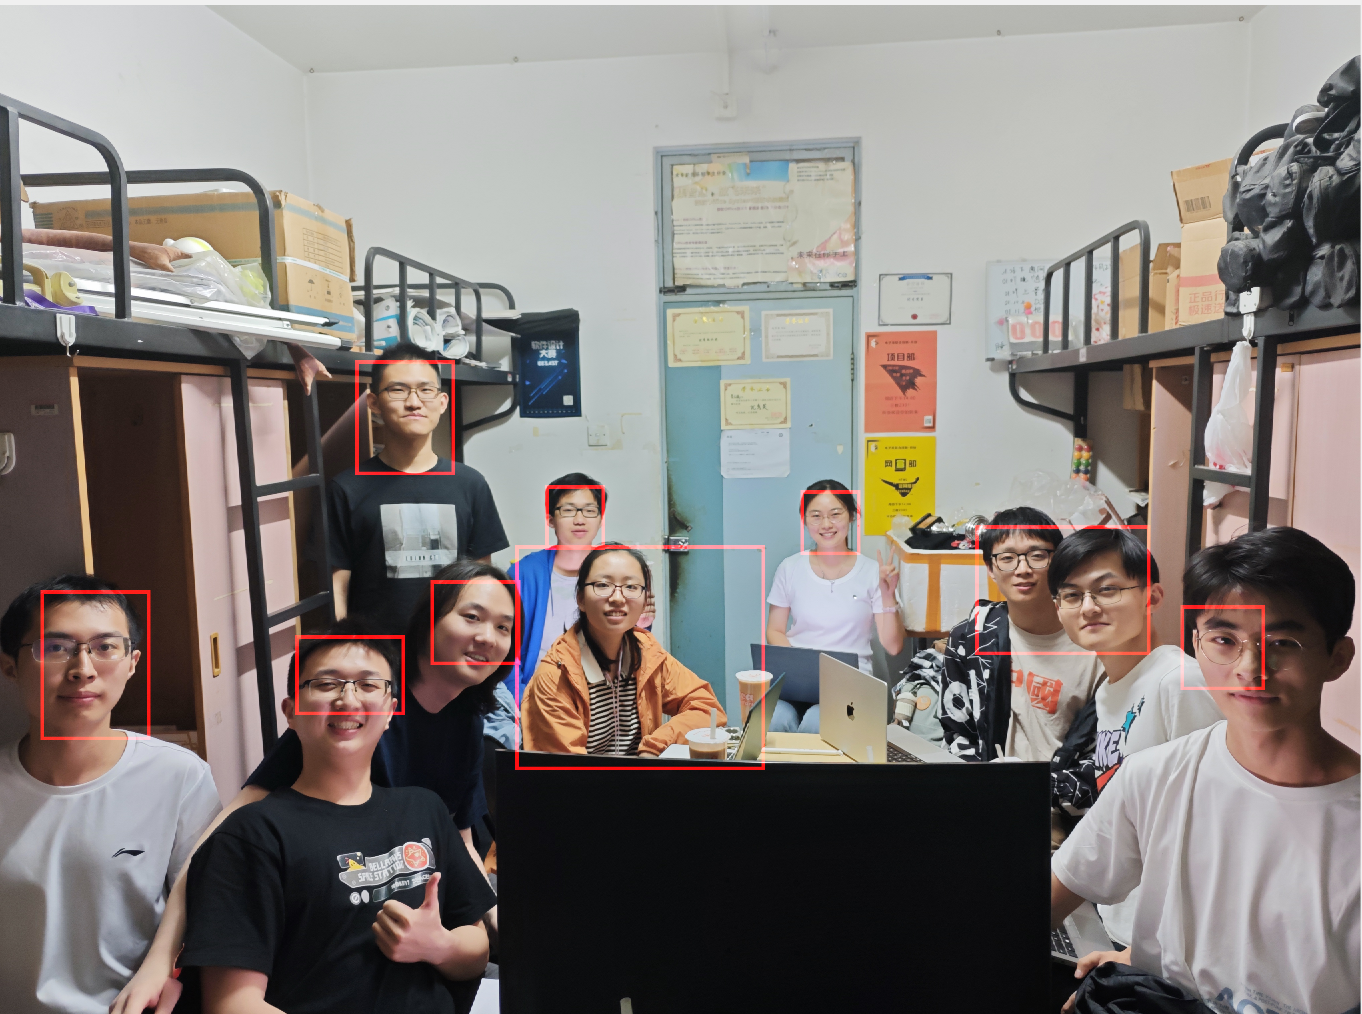
\includegraphics[width=0.6\linewidth]{shibie2.png}
    \caption{识别2}
\end{figure}

进一步调整参数,可以看到效果好了很多

\subsubsection{优化2:分割合并的人脸}
\textbf{采用kmeans聚类算法进行分割合并的人脸,具体算法如下:}
\begin{lstlisting}
    draw_rectangle = false(size(img_in));
    for i = 1 : 1 : n
        % 如果当前连通区域被标记为不需要处理,则跳过
        if flags(i) == 0
            continue;
        end
        % 找出属于当前连通区域的所有单元
        region_units = find(labs == i);
        [region_rows, region_cols] = ind2sub(size(labs), region_units);

        % 将单元坐标组合成一个矩阵
        unit_coords = [region_rows, region_cols];
        
        % 使用K-means聚类(假设最多分为2个矩形)
        [idx, centroids] = kmeans(unit_coords, 2);

        % 设置距离阈值
        distance_threshold = 16;
        
        % 判断是否需要分割
        % 如果确实分成了两类
        if size(unique(idx, 'rows'), 1) > 1 && pdist(centroids) >= distance_threshold
            rectangles = [];
            for k = 1:2
                cluster_units = unit_coords(idx == k, :);
                
                % 为每个聚类计算新的边界
                new_min_left = min(cluster_units(:, 2));
                new_min_top = min(cluster_units(:, 1));
                new_max_right = max(cluster_units(:, 2));
                new_max_bottom = max(cluster_units(:, 1));
                
                % 添加矩形信息
                rectangles = [rectangles; new_min_left, new_min_top, ...
                new_max_right, new_max_bottom];
            end
            rectangles = reshape(rectangles, [], 4);
            % 绘制矩形
            for r = 1:size(rectangles, 1)
                top_start = (rectangles(r, 2) - 1) * h_step + 1;
                bottom_end = rectangles(r, 4) * h_step;
                left_start = (rectangles(r, 1) - 1) * w_step + 1;
                right_end = rectangles(r, 3) * w_step;
                
                draw_rectangle(top_start : bottom_end, ...
                left_start : left_start + line_width) = true;
                draw_rectangle(top_start : top_start + line_width, ...
                left_start: right_end) = true;
                draw_rectangle(top_start: bottom_end, ...
                max(1, right_end - line_width) : right_end) = true;
                draw_rectangle(max(1, bottom_end - line_width) : bottom_end, ... 
                left_start : right_end) = true;
            end
        else
            % 绘制矩形
            top_start = (min_top(i) - 1) * h_step + 1;
            bottom_end = max_bottom(i) * h_step;
            left_start = (min_left(i) - 1) * w_step + 1;
            right_end = max_right(i) * w_step;
            draw_rectangle( top_start : bottom_end, ...  
            left_start : left_start + line_width) = true;
            draw_rectangle( top_start : top_start + line_width, ... 
            left_start: right_end) = true;
            draw_rectangle( top_start: bottom_end, ... 
            max(1, right_end - line_width) : right_end) = true;
            draw_rectangle(max(1, bottom_end - line_width) : bottom_end, ... 
             left_start : right_end) = true;
        end
    end
\end{lstlisting}

效果如图:
\begin{figure}[H]
    \centering
    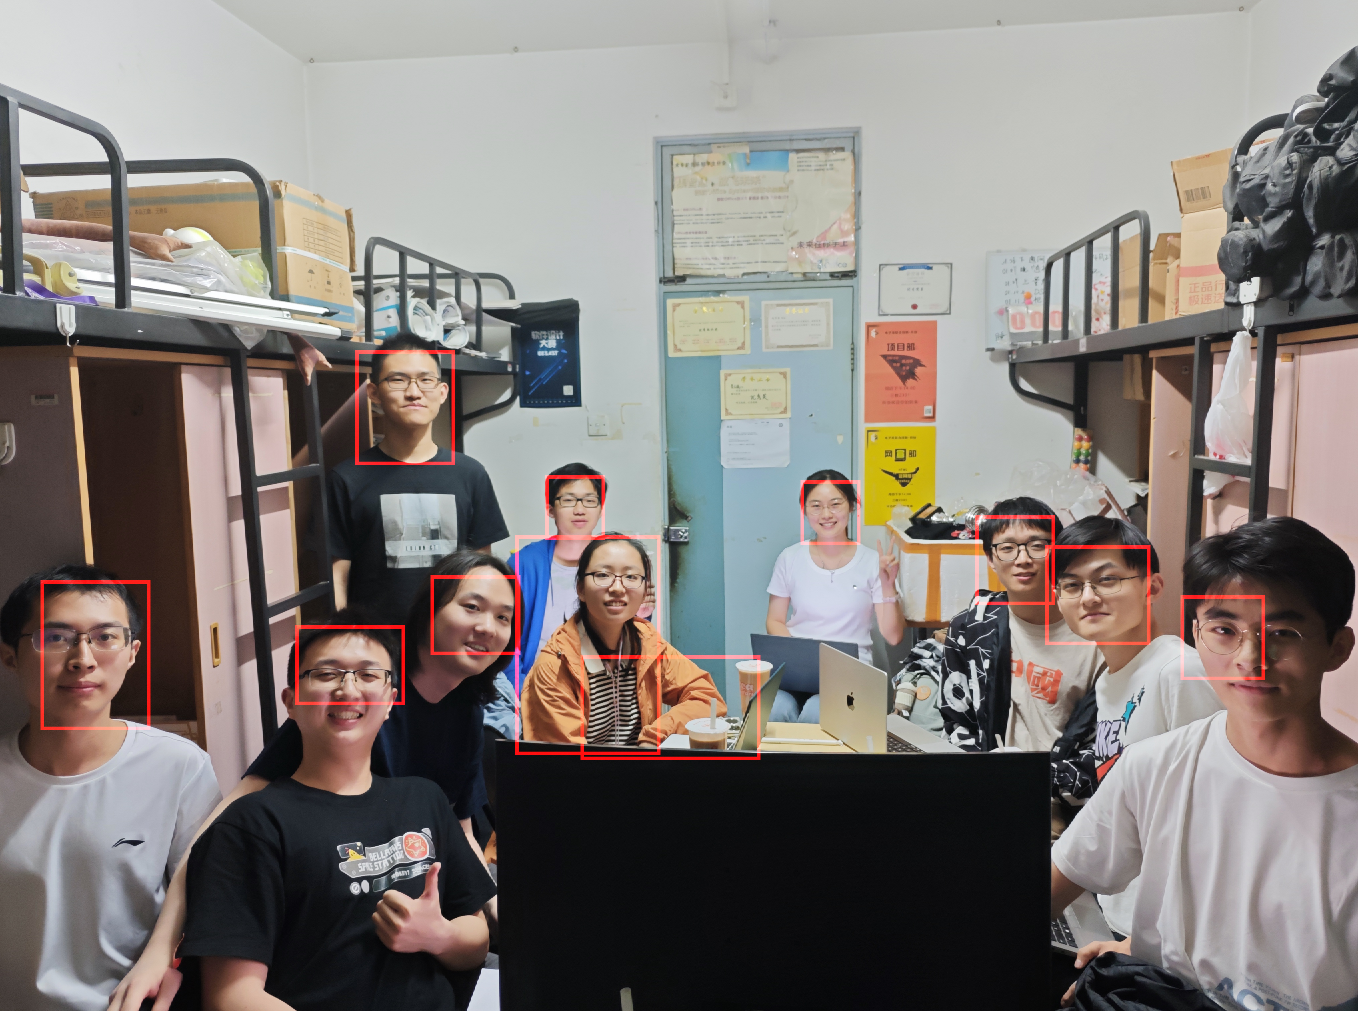
\includegraphics[width=0.6\linewidth]{shibie3.png}
    \caption{识别3}
\end{figure}
由于中间黄衣女生的衣服颜色和人脸颜色相近,导致识别效果不好,但是已经比之前好很多

\subsubsection{优化3:处理重叠矩形}
需要注意的是,当两个矩形重叠区域很小时不需要处理,如上图所示,因此我们检测,当两个矩形重叠区域大于一定阈值后再进行合并;
同时,合并并不是简单的取两个矩形的边界作为新边界,需要根据两个矩形的形状大小进行调整、合并,具体算法如下:

\begin{lstlisting}
    % 检查两个矩形是否重叠
    overlap_threshold = 0.3;  % 重叠阈值,可以根据需要调整
    rect1 = rectangles(1, :);
    rect2 = rectangles(2, :);
    % 计算重叠区域
    x_overlap = max(0, min(rect1(3), rect2(3)) - max(rect1(1), rect2(1)));
    y_overlap = max(0, min(rect1(4), rect2(4)) - max(rect1(2), rect2(2)));
    overlap_area = x_overlap * y_overlap;
    
    % 计算两个矩形的面积
    area1 = (rect1(3) - rect1(1) + 1) * (rect1(4) - rect1(2) + 1);
    area2 = (rect2(3) - rect2(1) + 1) * (rect2(4) - rect2(2) + 1);
    
    % 计算重叠比例(相对于较小的矩形)
    min_area = min(area1, area2);
    overlap_ratio = overlap_area / min_area;
    
    if overlap_ratio > overlap_threshold
        % 如果重叠比例大于阈值,合并两个矩形
        merged_rect = [
            min(rect1(1), rect2(1));  % 最小左边界
            min(rect1(2), rect2(2));  % 最小上边界
            max(rect1(3), rect2(3));  % 最大右边界
            max(rect1(4), rect2(4))   % 最大下边界
        ];
        
        % 计算合并矩形的中心
        center_x = (merged_rect(1) + merged_rect(3)) / 2;
        center_y = (merged_rect(2) + merged_rect(4)) / 2;
        
        % 计算合并矩形的宽度和高度
        width = merged_rect(3) - merged_rect(1) + 1;
        height = merged_rect(4) - merged_rect(2) + 1;
        
        % 调整合并矩形的大小,使其更接近原始矩形的平均大小
        avg_width = (rect1(3) - rect1(1) + rect2(3) - rect2(1) + 2) / 2;
        avg_height = (rect1(4) - rect1(2) + rect2(4) - rect2(2) + 2) / 2;
        
        adjusted_width = (width + avg_width) / 2;
        adjusted_height = (height + avg_height) / 2;
        
        % 计算调整后的矩形边界
        adjusted_rect = [
            max(1, round(center_x - adjusted_width / 2)),
            max(1, round(center_y - adjusted_height / 2)),
            min(w_num, round(center_x + adjusted_width / 2)),
            min(h_num, round(center_y + adjusted_height / 2))
        ];
        rectangles = adjusted_rect;
    end
\end{lstlisting}

最终效果如图,黄衣女生的衣服与人脸颜色矢量过于相似,难以去除,除此之外整体效果不错:

\begin{figure}[H]
    \centering
    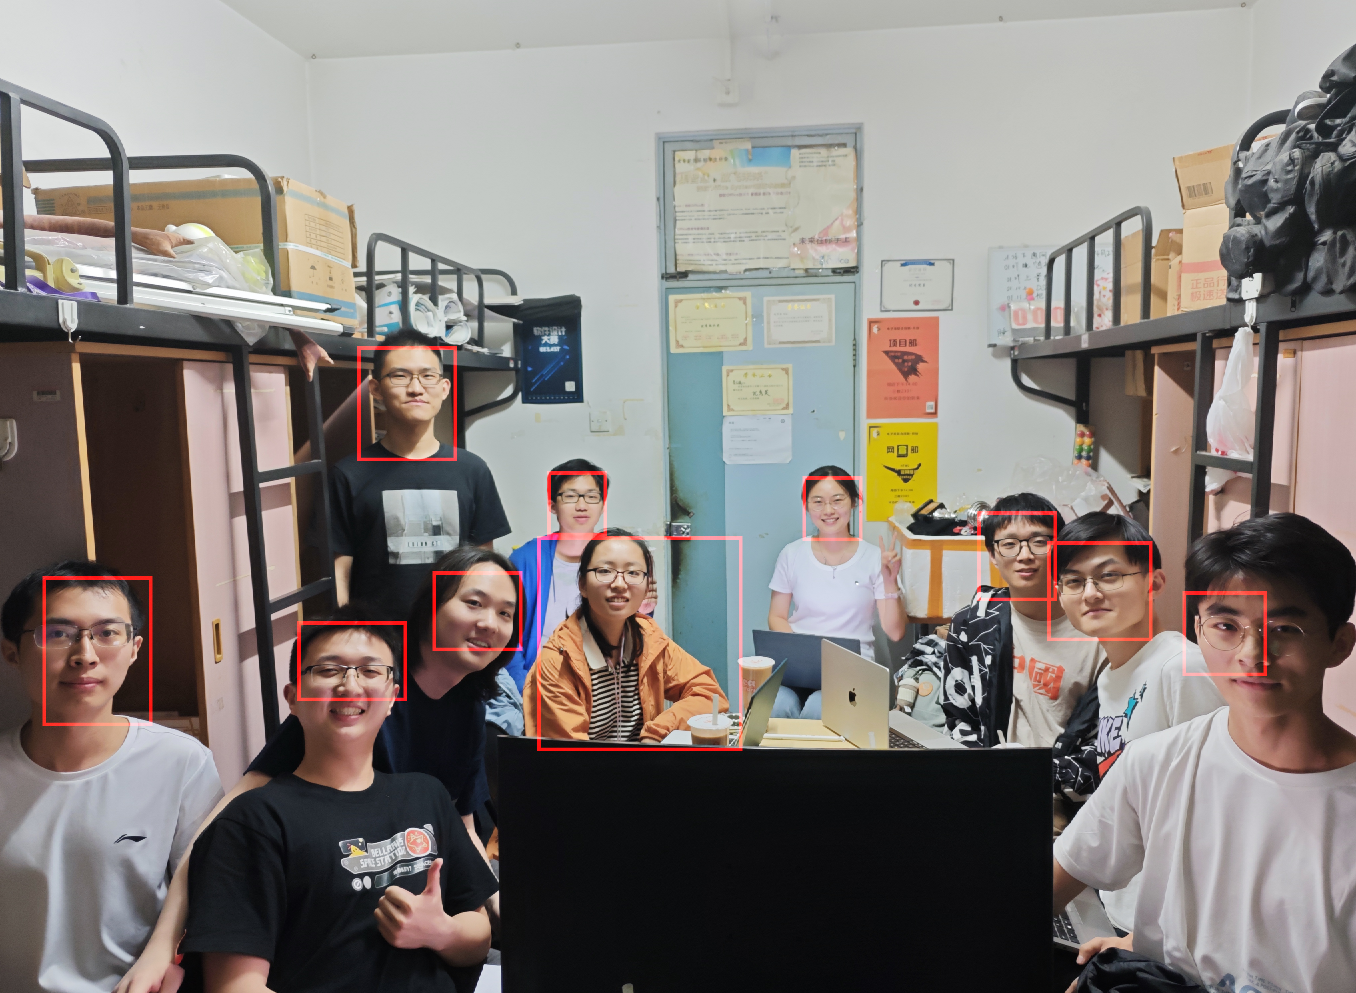
\includegraphics[width=0.6\linewidth]{shibie4.png}
    \caption{识别4}
\end{figure}

局限性:\\
1. 对于明暗不一的图像效果不好,矩形无法完全框住人脸\\
2. 对于人体其他部位干扰的图像效果不好\\

由于现有算法基于颜色矢量,且人脸样本较为单一,数量较少,上述问题很难解决,如果将人脸轮廓作为参数进行识别,效果可能会更好

\subsubsection{分别取不同的L进行识别}
\begin{figure}[H]
    \centering
    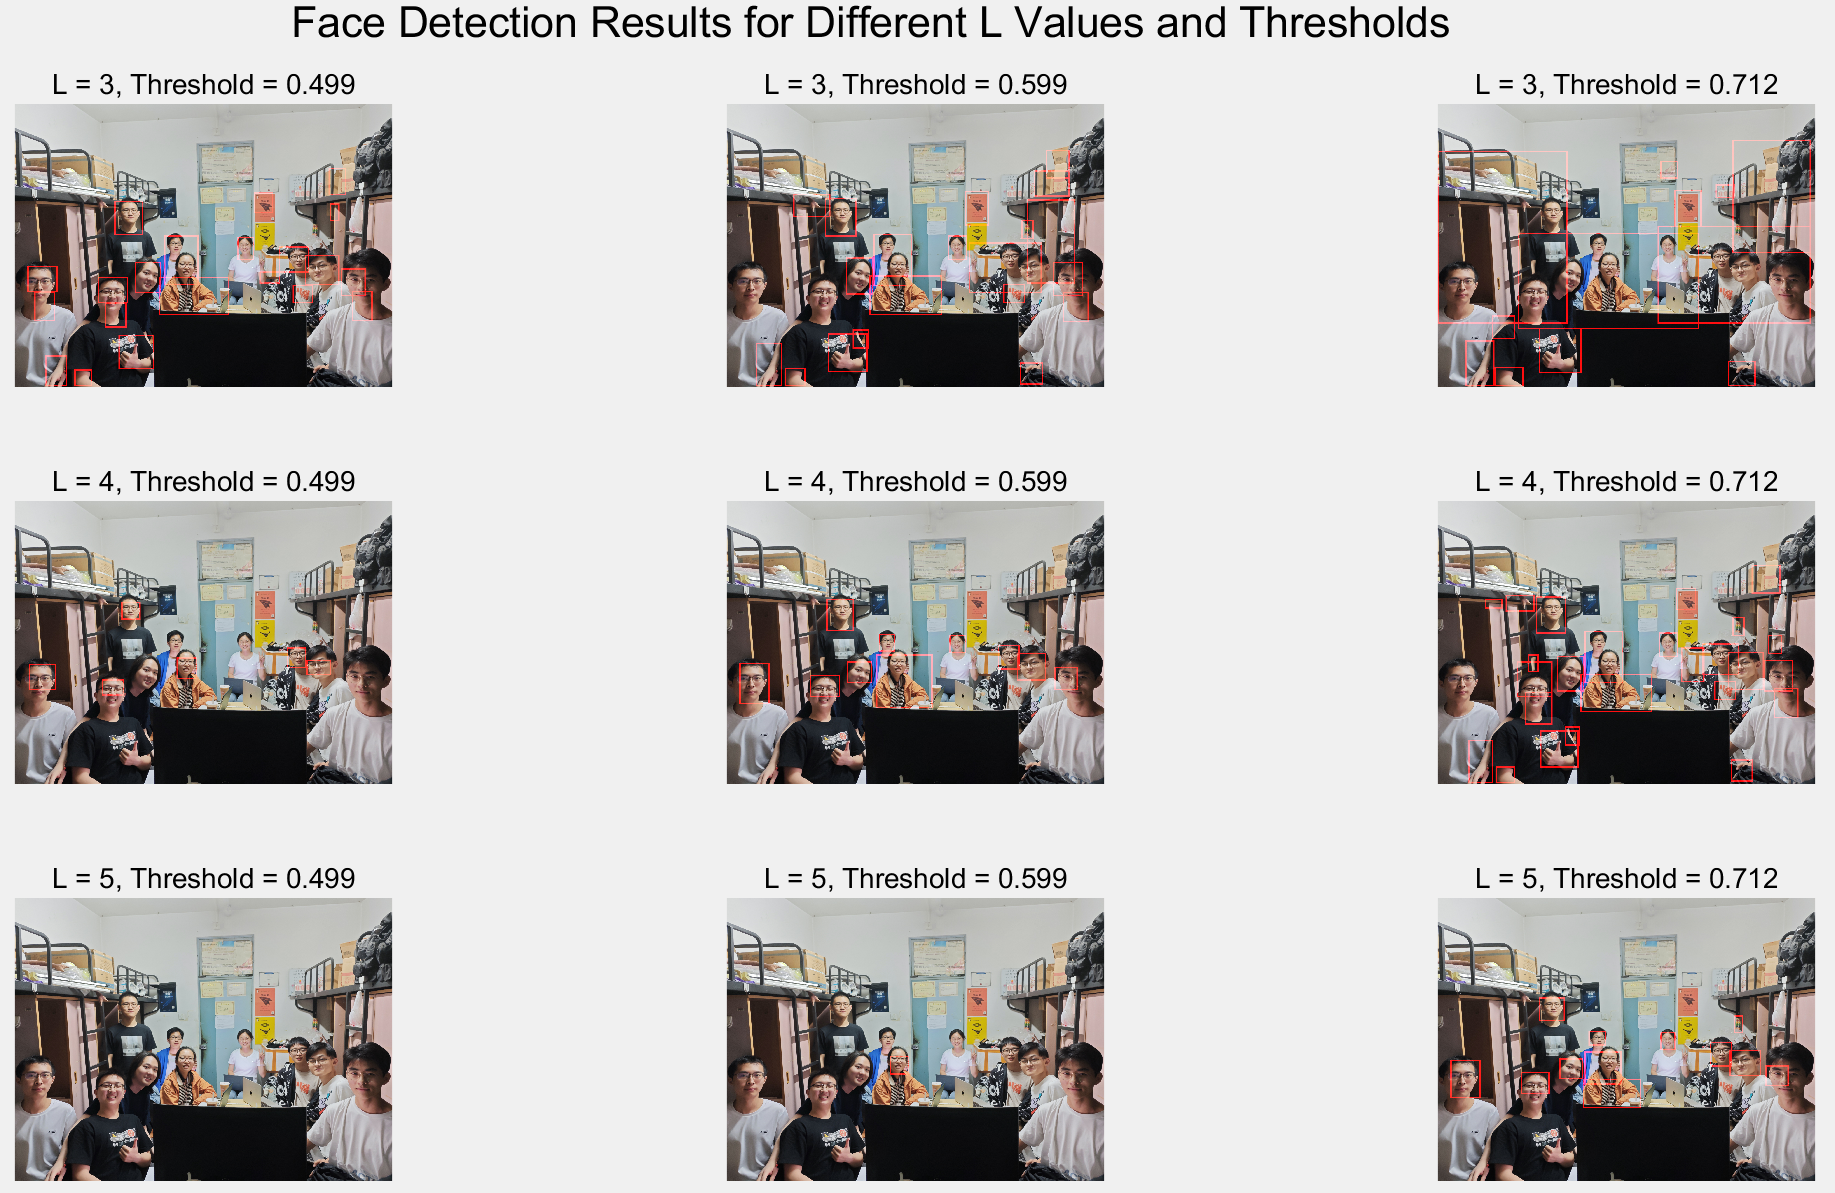
\includegraphics[width=0.9\linewidth]{shibie5.png}
    \caption{识别5}
\end{figure}
可以看到,在现有的算法下,当L过大时,所需要的阈值更大,对图像更敏感,容易出现检测不到人脸的情况;当L过小时,
所需要的阈值更小,对图像更不敏感,容易出现更复杂的矩形重叠情况,识别效果很差\\
\hspace*{2em}可以在附件中看到更清晰的效果图

\subsection{对图像处理后再进行人脸识别}
\subsubsection{顺时针旋转90度}
效果如图:
\begin{figure}[H]
    \centering
    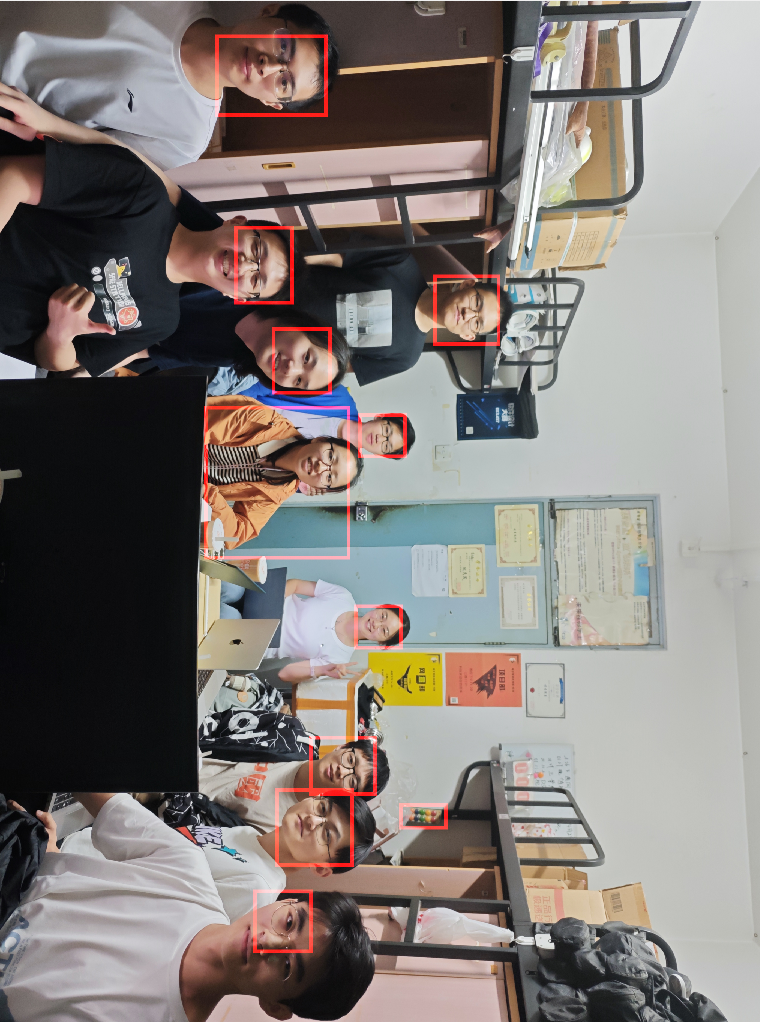
\includegraphics[width=0.4\linewidth]{rotate.png}
    \caption{顺时针旋转90度}
\end{figure}
可以看到识别效果基本没有变化,说明算法对旋转不敏感
\subsubsection{保持高度不变,宽度拉伸为原来的2倍}
\begin{figure}[H]
    \centering
    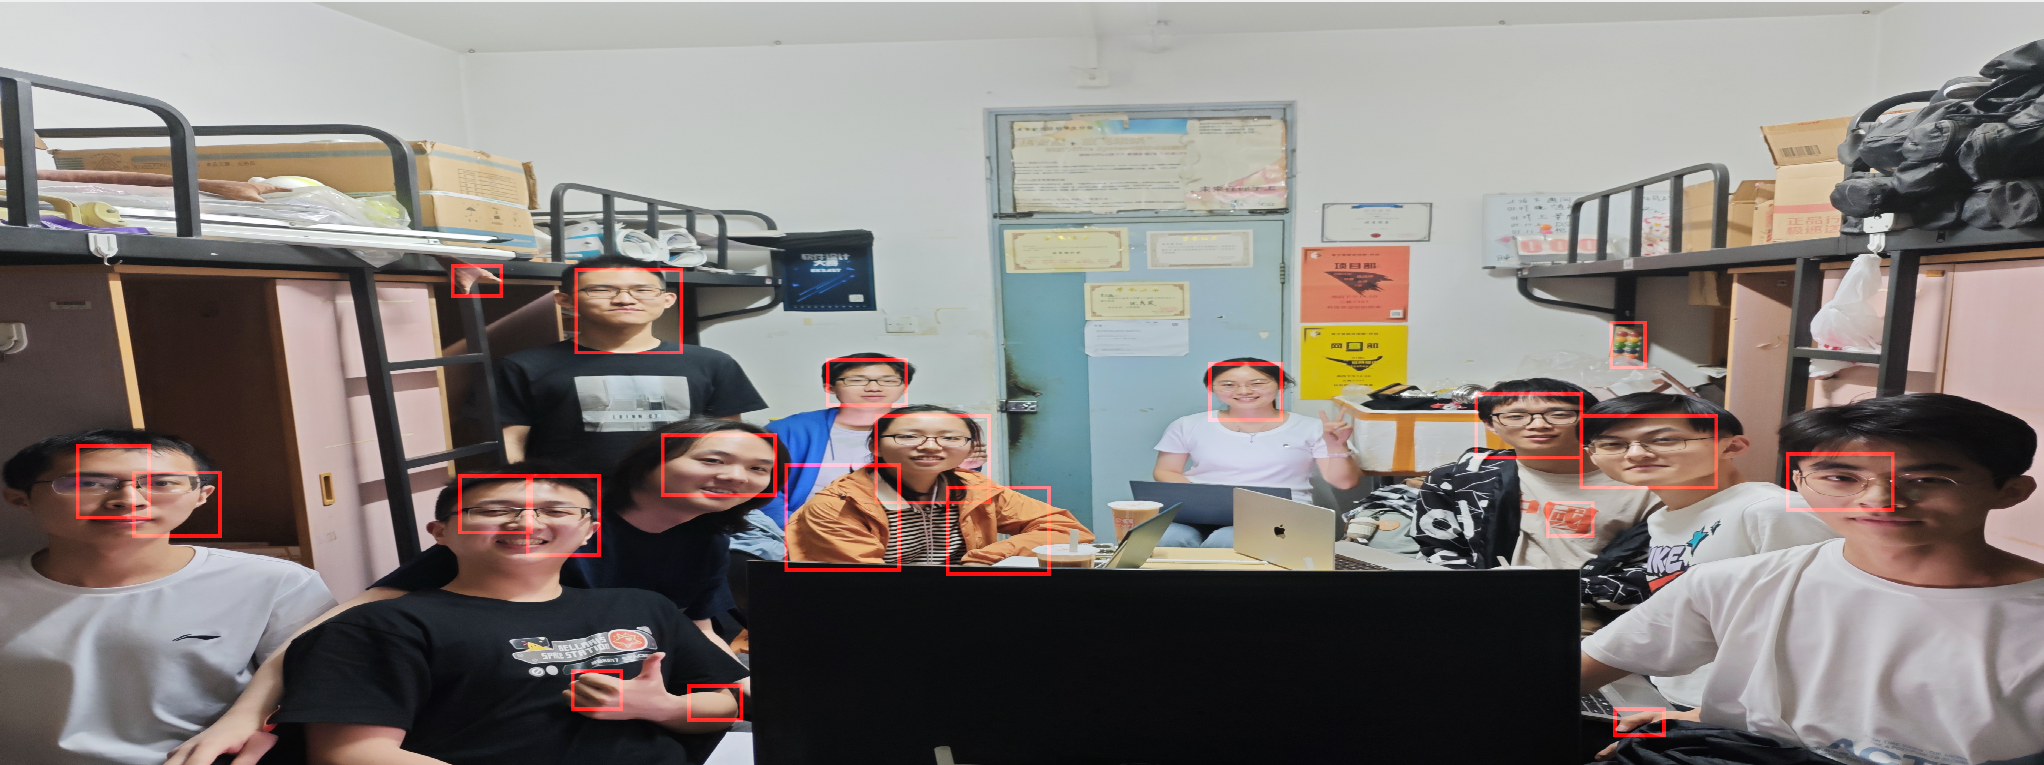
\includegraphics[width=0.8\linewidth]{stretch.png}
    \caption{宽度拉伸2倍}
\end{figure}
可以看到出现了小矩形未过滤和矩形不合理的分割的情况,原因在于拉伸后原有的距离阈值不适用,调整参数后就可以正常识别,说明此算法对宽度拉伸较为敏感
\subsubsection{适当改变颜色}
1. 调暗图片
\begin{figure}[H]
    \centering
    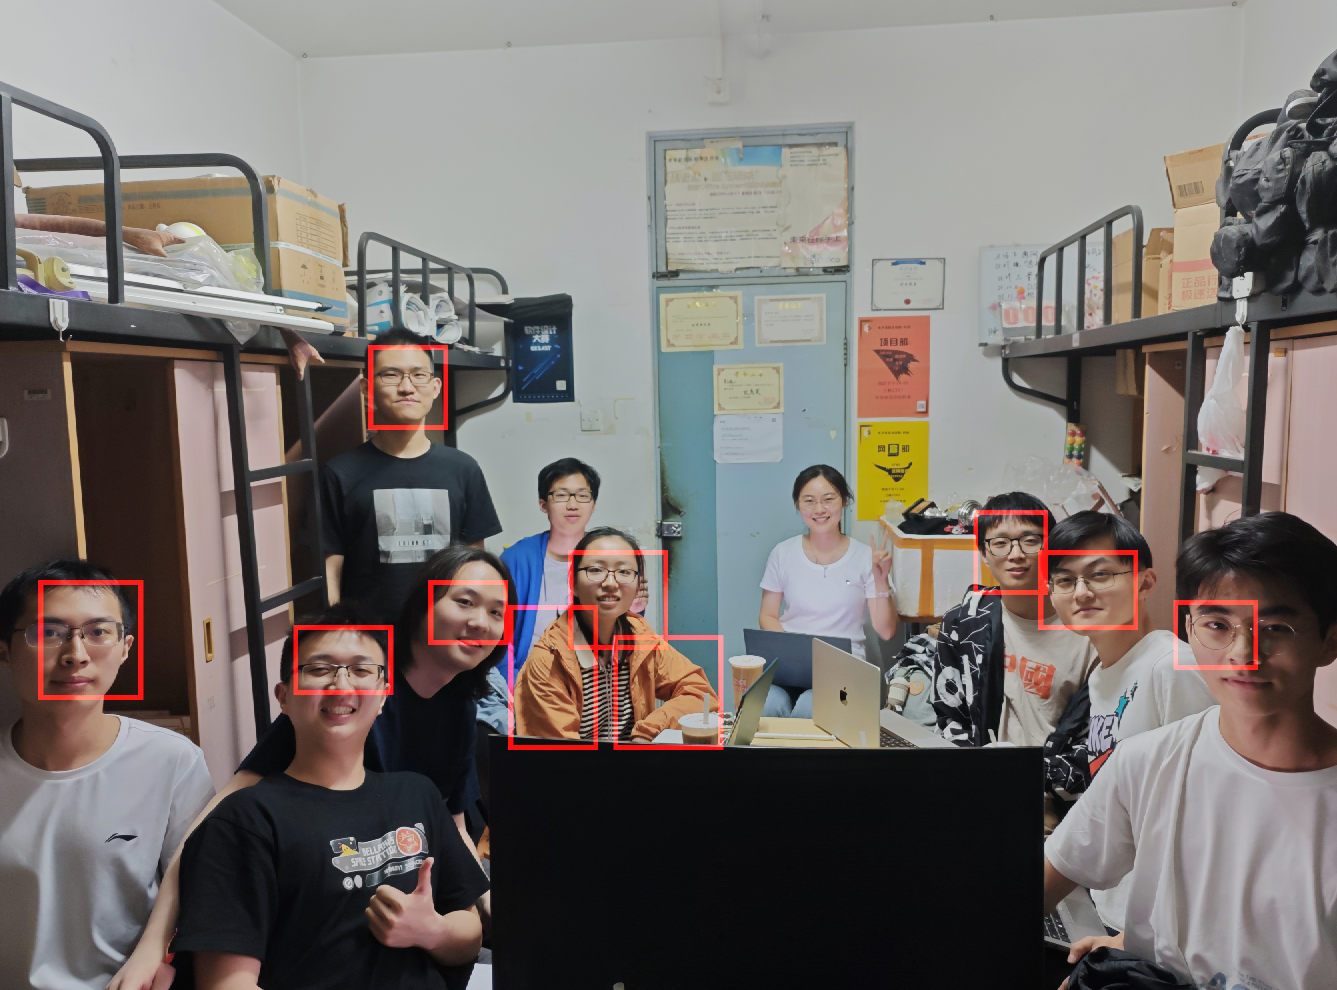
\includegraphics[width=0.6\linewidth]{dark.png}
    \caption{调暗图片}
\end{figure}
2. 调亮图片
\begin{figure}[H]
    \centering
    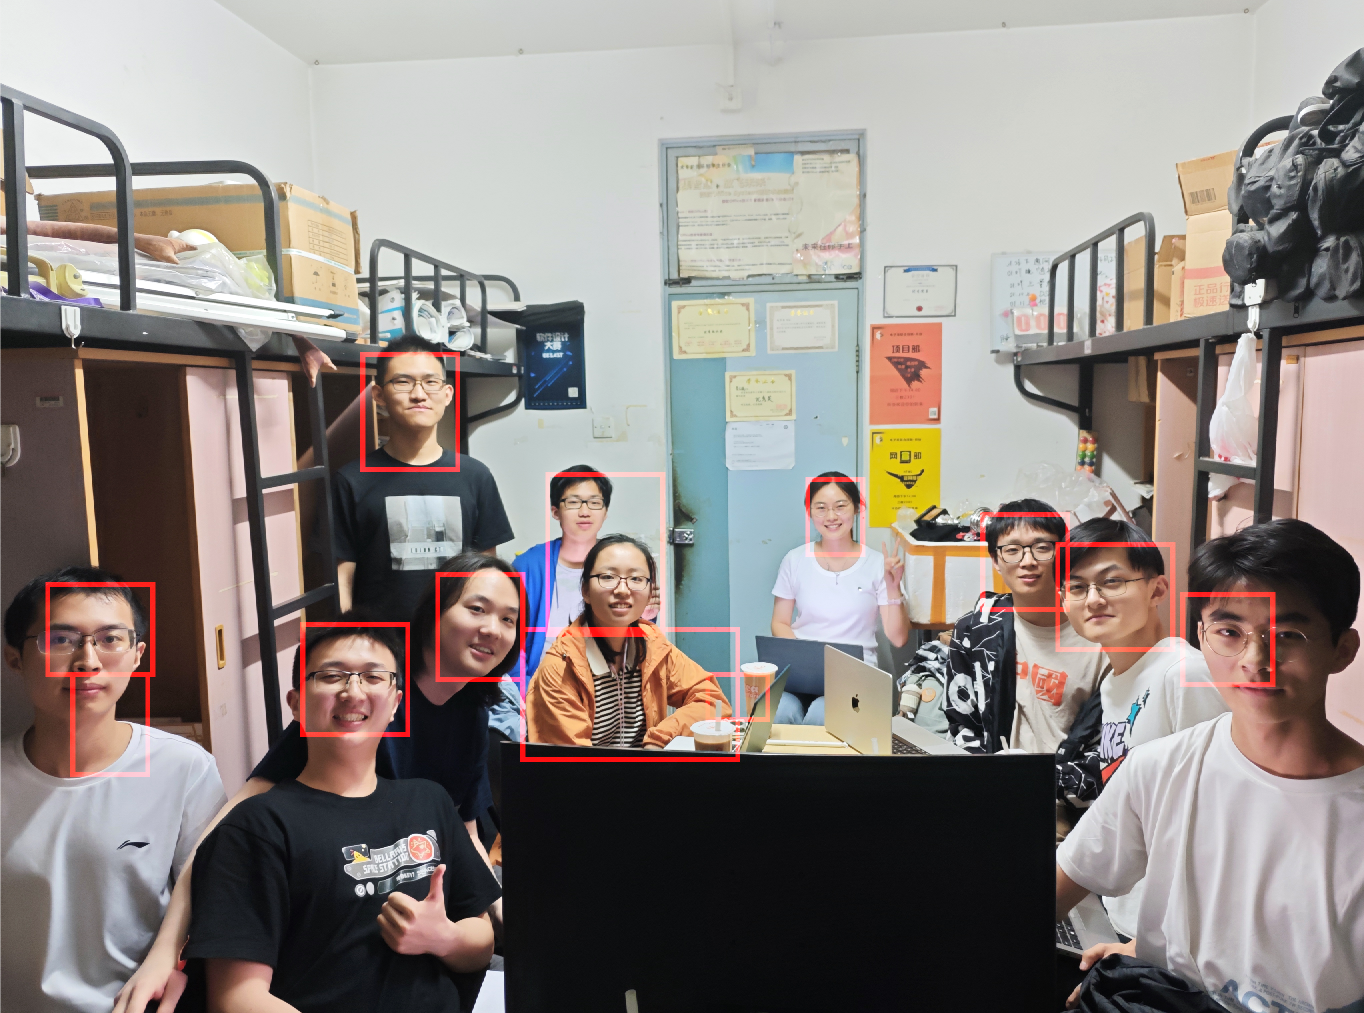
\includegraphics[width=0.6\linewidth]{bright.png}
    \caption{调亮图片}
\end{figure}
可以看到调暗图片后部分人脸没有识别出来,而调亮图片后识别结果变化不大,推测原因在于训练图片的亮度大于测试图片,因此调低测试图片的亮度会带来更大的误差
\subsection{重新选择人脸标准}

从上面的实验可以看出,仅通过颜色矢量进行人脸识别效果并不好,因此将人脸轮廓纳入识别参数可能会更好,而且应该选择更多丰富的样本,包括不同角度、不同光照、不同人种、
不同年龄的人脸样本,这样可以更好地适应不同的图像,提高识别效果

\section{版本借鉴情况}
说明:人脸识别部分的初版思路参考了9字班学长的\href{https://github.com/Timothy-Liuxf/THUEE_MATLAB/tree/master/image}{方法},但是在原有方法上有较大优化\\
\end{document}
